% Customizable fields and text areas start with % >> below.
% Lines starting with the comment character (%) are normally removed before release outside the collaboration, but not those comments ending lines

%%%%%%%%%%%%% local definitions %%%%%%%%%%%%%%%%%%%%%
\RCS$Revision: 438143 $
\RCS$HeadURL: svn+ssh://svn.cern.ch/reps/tdr2/notes/AN-16-395/trunk/AN-16-395.tex $
\RCS$Id: AN-16-395.tex 438143 2017-12-08 13:49:18Z fjensen $

\newcommand{\invfb}{\fbinv}
\newcommand{\invpb}{\pbinv}
\newcommand{\met}{\MET}
\newcommand{\MHT}{\ensuremath{\rm{H}_{\rm{T}}^{miss}}}
\newcommand{\gluino}{\ensuremath{\tilde{g}}\xspace}
\newcommand{\NLSP}{\ensuremath{\tilde{\chi}^0_2}\xspace}
\newcommand{\dphi}{\ensuremath{\Delta \phi_{\mathrm{min}}}\xspace}
\newcommand{\LSP}{\ensuremath{\tilde{\chi}^0_1}\xspace}
\newcommand{\lsp}{\LSP}
\newcommand{\mgluino}{\ensuremath{m_{\sGlu}}\xspace}
\newcommand{\znn}{\ensuremath{\Z\rightarrow \nu\overline{\nu}}\xspace}
\newcommand{\hbb}{\ensuremath{H\rightarrow b\overline{b}}\xspace}
\newcommand{\lint}{\ensuremath{\int\lumi\,\rd{t}}\xspace}
% This allows for switching between one column and two column (cms@external) layouts
% The widths should  be modified for your particular figures. You'll need additional copies if you have more than one standard figure size.
\newlength\cmsFigWidth
\ifthenelse{\boolean{cms@external}}{\setlength\cmsFigWidth{0.85\columnwidth}}{\setlength\cmsFigWidth{0.4\textwidth}}
\ifthenelse{\boolean{cms@external}}{\providecommand{\cmsLeft}{top\xspace}}{\providecommand{\cmsLeft}{left\xspace}}
\ifthenelse{\boolean{cms@external}}{\providecommand{\cmsRight}{bottom\xspace}}{\providecommand{\cmsRight}{right\xspace}}
%%%%%%%%%%%%%%%  Title page %%%%%%%%%%%%%%%%%%%%%%%%
\cmsNoteHeader{AN-19-025} % This is over-written in the CMS environment: useful as preprint no. for export versions
% >> Title: please make sure that the non-TeX equivalent is in PDFTitle below for papers. For PASs, PDFTitle can be used with plain TeX.
\title{Search for supersymmetry using boosted Z Bosons and
missing transverse momentum in proton-proton collisions
at 13 TeV}

% >> Authors
%Author is always "The CMS Collaboration" for PAS and papers, so author, etc, below will be ignored in those cases
%For multiple affiliations, create an address entry for the combination
%To mark authors as primary, use the \author* form
\address[COL]{University of Colorado Boulder (US)}
\address[TIFR]{Tata Institute of Fundamental Research, Mumbai}
\author[COL]{R.~Patel}
\author[TIFR]{U.~Sarkar}
% >> Date
% The date is in yyyy/mm/dd format. Today has been
% redefined to match, but if the date needs to be fixed, please write it in this fashion.
\date{\today}

% >> Abstract
% Abstract processing:
% 1. **DO NOT use \include or \input** to include the abstract: our abstract extractor will not search through other files than this one.
% 2. **DO NOT use %**                  to comment out sections of the abstract: the extractor will still grab those lines (and they won't be comments any longer!).
% 3. For PASs: **DO NOT use CMS tex macros.**...in the abstract: CDS MathJax processor used on the abstract doesn't understand them _and_ will only look within $$. The abstracts for papers are hand formatted so macros are okay.
\abstract{
   A search for supersymmetry is presented with bosons and large missing transverse momentum in proton-proton collisions collected by the CMS experiment at the LHC at $\sqrt{s}=13$~TeV. We target Higgs bosons produced with large momentum, where the hadronization byproducts of a pair of b-quarks can be reconstructed in a single jet. The analysis makes use of an algorithm to identify jets reconstructed from overlapping $b\overline{b}$. The background from multijet and $t\overline{t}$ events is significanctly reduced with requirements on the heavy flavor tagging of the jet and its mass. The data sample corresponds to an integrated luminosity of 35.9~fb$^{-1}$ and was collected in 2016.
}

% >> PDF Metadata
% Do not comment out the following hypersetup lines (metadata). They will disappear in NODRAFT mode and are needed by CDS.
% Also: make sure that the values of the metadata items are sensible and are in plain text with the possible exception of the PDFtitle for a PAS. Then you can use pure TeX symbols as if on a typewriter. Examples: $\sqrt{s}=13\TeV$ => $sqrt{s}=$ 13 TeV; 32\fbinv => 32 fb$^{-1}$
% No unescaped comment % characters.
% No curly braces {} except for TeX in the PDFtitle.
\hypersetup{%
pdfauthor={CMS Collaboration},%
pdftitle={Search for supersymmetry using boosted Z Bosons and
missing transverse momentum in proton-proton collisions
at 13 TeV},%
pdfsubject={CMS},%
pdfkeywords={CMS, physics, software, computing}}

\maketitle %maketitle comes after all the front information has been supplied
% >> Text
%%%%%%%%%%%%%%%%%%%%%%%%%%%%%%%%  Begin text %%%%%%%%%%%%%%%%%%%%%%%%%%%%%
%% **DO NOT REMOVE THE BIBLIOGRAPHY** which is located before the appendix.
%% You can take the text between here and the bibiliography as an example which you should replace with the actual text of your document.
%% If you include other TeX files, be sure to use "\input{filename}" rather than "\input f
\clearpage
\tableofcontents
\clearpage

\section{Introduction}
\label{sec:introduction}


\section{Event samples}
\label{sec:event-samples}

\subsection{Standard model MC samples}
\label{sec:sm-mc}
Monte Carlo (MC) samples reconstructed with CMSSW release 8\_0\_X (Summer16) are used for all processes. The SM samples are listed in Tables \ref{tab:ttbarMCsamples}, \ref{tab:qcdMCsamples}, \ref{tab:zjetsMCsamples}, and \ref{tab:wjetsMCsamples}.
The cross sections listed correspond to next-to-next-to-leading-order (NNLO) calculations
unless otherwise noted.  All samples use the PU25bx25 pileup scenario, which simulates a
pileup distribution with an average of 25 interactions per
bunch crossing and a 25 ns interval between bunches.
\begin{table}[hp!]
\centering
\caption{SM $t\bar{t}$ MC samples used in the analysis. The cross
  sections are calculated to NNLO. }
\label{tab:ttbarMCsamples}
{\footnotesize
\begin{tabular}{lcc}
\hline \hline
Dataset & $\sigma$ (pb) & \lint (fb$^{-1}$) \\
\hline
%TTJets\_TuneCUETP8M1\_13TeV-madgraphMLM-pythia8 & 831.76 & 12.34\\
TTJets\_SingleLeptFromT\_TuneCUETP8M1\_13TeV-madgraphMLM-pythia8 & 182.72 & 283.90\\
TTJets\_SingleLeptFromTbar\_TuneCUETP8M1\_13TeV-madgraphMLM-pythia8 & 182.72 & 326.48\\
TTJets\_DiLept\_TuneCUETP8M1\_13TeV-madgraphMLM-pythia8 & 88.34 & 346.25\\
TTJets\_HT-600to800\_TuneCUETP8M1\_13TeV-madgraphMLM-pythia8 & 2.734 & 5231.81\\
TTJets\_HT-800to1200\_TuneCUETP8M1\_13TeV-madgraphMLM-pythia8 & 1.121 & 9416.61\\
TTJets\_HT-1200to2500\_TuneCUETP8M1\_13TeV-madgraphMLM-pythia8 & 0.198 & 14819.34\\
TTJets\_HT-2500toInf\_TuneCUETP8M1\_13TeV-madgraphMLM-pythia8 & 0.002 & 221088.29\\
\hline \hline
\end{tabular}
}
\end{table}

\begin{table}[hp!]
\centering
\caption{SM QCD MC samples used in the analysis. All cross
  sections are calculated to LO.}
\label{tab:qcdMCsamples}
{\footnotesize
\begin{tabular}{lcc}
\hline \hline
Dataset & $\sigma$ (pb) & \lint (fb$^{-1}$) \\
\hline
QCD\_HT200to300\_TuneCUETP8M1\_13TeV-madgraphMLM-pythia8 & 1735000 & 0.03\\
QCD\_HT300to500\_TuneCUETP8M1\_13TeV-madgraphMLM-pythia8 & 366800 & 0.16\\
QCD\_HT500to700\_TuneCUETP8M1\_13TeV-madgraphMLM-pythia8 & 29370 & 1.95\\
QCD\_HT700to1000\_TuneCUETP8M1\_13TeV-madgraphMLM-pythia8 & 6524 & 6.68\\
QCD\_HT1000to1500\_TuneCUETP8M1\_13TeV-madgraphMLM-pythia8 & 1064 & 12.62\\
QCD\_HT1500to2000\_TuneCUETP8M1\_13TeV-madgraphMLM-pythia8 & 121.5 & 32.63\\
QCD\_HT2000toInf\_TuneCUETP8M1\_13TeV-madgraphMLM-pythia8 & 25.42 & 239.30\\
\hline \hline
\end{tabular}
}
\end{table}

\begin{table}[hp!]
\centering
\caption{SM $Z\rightarrow\nu\nu+$jets MC samples used in the analysis. The cross
  sections are calculated to NNLO. }
\label{tab:zjetsMCsamples}
{\footnotesize
\begin{tabular}{lcc}
\hline \hline
Dataset & $\sigma$ (pb) & \lint (fb$^{-1}$) \\
\hline
ZJetsToNuNu\_HT-100To200\_13TeV-madgraph & 344.8 & 54.13\\
ZJetsToNuNu\_HT-200To400\_13TeV-madgraph & 95.53 & 208.46\\
ZJetsToNuNu\_HT-400To600\_13TeV-madgraph & 13.20 & 77.30\\
ZJetsToNuNu\_HT-600To800\_13TeV-madgraph & 3.148 & 1795.26\\
ZJetsToNuNu\_HT-800To1200\_13TeV-madgraph & 1.451 & 1486.09\\
ZJetsToNuNu\_HT-1200To2500\_13TeV-madgraph & 0.355 & 1029.81\\
ZJetsToNuNu\_HT-2500ToInf\_13TeV-madgraph & 0.0085 & 47498.87\\
\hline \hline
\end{tabular}
}
\end{table}
\begin{table}[hp!]
\centering
\caption{SM $W\rightarrow\ell\nu+$jets MC samples used in the analysis. The cross
  sections are calculated to NNLO. }
\label{tab:wjetsMCsamples}
{\footnotesize
\begin{tabular}{lcc}
\hline \hline
Dataset & $\sigma$ (pb) & \lint (fb$^{-1}$) \\
\hline
WJetsToLNu\_HT-100To200\_TuneCUETP8M1\_13TeV-madgraphMLM-pythia8 & 1627.45 & 18.16\\
WJetsToLNu\_HT-200To400\_TuneCUETP8M1\_13TeV-madgraphMLM-pythia8 & 435.24 & 45.88\\
WJetsToLNu\_HT-400To600\_TuneCUETP8M1\_13TeV-madgraphMLM-pythia8 & 59.18 & 123.64\\
WJetsToLNu\_HT-600To800\_TuneCUETP8M1\_13TeV-madgraphMLM-pythia8 & 14.58 & 221.32\\
WJetsToLNu\_HT-800To1200\_TuneCUETP8M1\_13TeV-madgraphMLM-pythia8 & 6.66 & 1123.13\\
WJetsToLNu\_HT-1200To2500\_TuneCUETP8M1\_13TeV-madgraphMLM-pythia8 & 1.608 & 153.44\\
WJetsToLNu\_HT-2500ToInf\_TuneCUETP8M1\_13TeV-madgraphMLM-pythia8 & 0.039 & 6497.28\\
\hline \hline
\end{tabular}
}
\end{table}


\subsection{Signal models}
\label{sec:signal-models}

\begin{figure}[htbp!]
\centering
\includegraphics[width=0.20\linewidth]{plots/event-samples/T5ZZ.pdf}
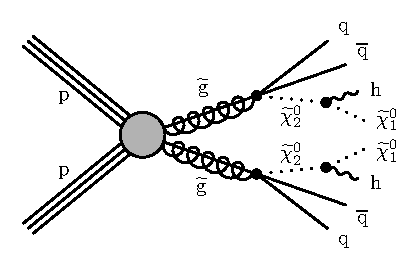
\includegraphics[width=0.20\linewidth]{plots/event-samples/T5hh.pdf}
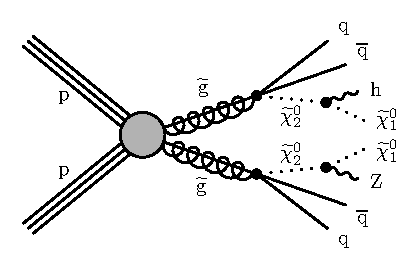
\includegraphics[width=0.20\linewidth]{plots/event-samples/T5Zh.pdf}
\caption{
Signal diagrams for the boosted Higgs search via gluino strong production. We consider 100$\%$ branching fraction to the Z boson(left).
}
\label{fig:T5-event-diagrams}
\end{figure}


Figure~\ref{fig:T5-event-diagrams} shows the event diagrams for the signal considered in this analysis. The mass splitting between \gluino and \NLSP is fixed at 50\gev, thus each of the \gluino produces a low \pt quark. The mass of the \LSP is fixed to 1\gev so that the Z boson \pt is proportional to $m_{\NLSP}/2\sim m_{\gluino}/2$. The signal regions for this analysis are the events strictly with 2 Z bosons with 100$\%$ branching fraction in the final state, where $Z\rightarrow b\bar{b}$ or $Z\rightarrow\nu\bar{\nu}$. For most gluino masses, the b-quarks, $Z\rightarrow b\bar{b}$ are expected to be contained in a large-radius jet, $\Delta R=0.8$ instead of showing up as two resolved jets due to the boosted topology of the model. Events are generated with the Full Simulation using the reconstruction in CMSSW version \texttt{8\_0\_X}.


\def \triggerPlotsDir {plots/triggers/}
\section{Triggers}
\label{sec:trigger}
In Section~\ref{sec:event-selection}, the primary offline kinematic selection for the search region is $H_{T}>500$\gev and $\met>300$\gev,along with vetoed the events with leptons. This section will describe the trigger efficiency for the signal and control regions, and check if these offline regions are well above the trigger turn-on.

\subsection{Signal region}
\label{sec:signalTriggers}


\subsection{Single-$\mu$ region}
\label{sec:SingleMuTrig}

\subsection{Single-e region}


\subsection{Single-photon region}
\label{sec:photonTrg}
  
%\begin{table} 
%\centering
%\caption{Low-$\Delta\phi$ trigger efficiencies ($\%$).}
%\label{table:lowDphiEff}
%\begin{tabular}{c|c|c} 
%\hline \hline
% 100$<$\MET$<$200 & 200$<$\MET$<$300 & 300$<$\MET$<$400 \\
%\hline \hline
%50.0$_{-0.1}^{+0.1}$ & 71.2$_{-0.1}^{+0.1}$ & 80.6$_{-0.2}^{+0.2}$ \\ \hline \hline
%400$<$\MET$<$500 & 500$<$\MET$<$700 & \MET$>$700 \\ \hline \hline
%87.4$_{-0.3}^{+0.3}$ & 86.6$_{-0.5}^{+0.4}$ & 76.6$_{-1.3}^{+1.2}$ \\ 
%\hline \hline
%\end{tabular}
%\end{table}


\section{Event selection}
\label{sec:event-selection}
Since the the final state of signal model is boosted and purely hadronic, the search regions for this analysis require large \MET, large \HT, and no leptons.
The selection makes use of the same kinematic variables as more inclusive SUSY analyses~\cite{RA2b:Moriond}.
Jets used in this analysis are reconstructed from charged-hadron subtracted particle-flow (PF) candidates using the anti-\kt algorithm~\cite{Cacciari:2008gp} with size parameters $0.8$ (AK8) and $0.4$ (AK4).
The PF algorithm is used to individually identify and reconstruct all particles produced in the collision (PF candidates); namely charged hadrons, photons, neutral hadrons, muons, and electrons~\cite{PF}.
Selection is applied to the AK8 jets to ensure a boosted topology and most likely to come from Z boson.
The AK8 jets are reclustered from their original jet constituents, and the clustering sequence is modified to remove soft and wide-angle particles or groups of particles. The reclustering method that has been used is softdrop.
This "softdrop jet" is used to compute the mass after removing the soft radiation to provide a narrower Z mass window~\cite{JetSub:Prune}. 
AK4 jets are used to compute the \HT, \MHT, and $\Delta\phi$ variables. 
The following requirements define the baseline selection:

\begin{itemize}

\item  $\HT > 500 \gev$, where $\HT = \sum_{\mathrm{AK4 jets}} \pt$ 
 \begin{itemize}
  \item AK4 jets are required to pass the loose jet ID requirements: \\
   For jets with $|\eta|<2.4$:
   \begin{itemize}
    \item neutral hadron fraction $<$ 0.99,
    \item neutral EM fraction $<$ 0.99,
    \item number of constituents $>$ 1,
    \item charged hadron fraction $>$ 0,
    \item charged multiplicity $>$ 0,
    \item charged EM fraction $<$ 0.99
   \end{itemize}
   %For jets with $2.4<|\eta|<2.7$:
   %\begin{itemize}
   %  \item neutral hadron fraction $<$ 0.99,
   %  \item neutral EM fraction $<$ 0.99,
   %  \item number of constituents $>$ 1,
   %\end{itemize}
   %For jets with $2.7<|\eta|<3.0$:
   %\begin{itemize}
   %  \item neutral EM fraction $<$ 0.90,
   %  \item number of neutral constituents $>$ 2,
   %\end{itemize}
   %For jets with $3.0<|\eta|<5.0$:
   %\begin{itemize}
   %  \item neutral EM fraction $<$ 0.90,
   %  \item number of neutral constituents $>$ 10,
   %\end{itemize}
   Within the validation regions, jets that are matched to isolated leptons, within $\Delta R<0.4$ are not subject to these requirements.   
 \end{itemize}

\item $\MET>300 \gev$ where $\MET = \left|\sum_{\mathrm{PF candidates}} \vec{p}_{T}\right|$.

\item $\MHT>200 \gev$ where $\MHT = \left|\sum_{\mathrm{AK4 jets}} \vec{p}_{T}\right|$.

\item To ensure events with a boosted topology, events are selected based on high \pt AK8 jets with the following criteria:
   \begin{itemize}
   \item Require the event to have at least two AK8 jets with leading jet\pt$>300$\gev and subleading jet\pt$>200$\gev
   \item The softdrop mass~\cite{Pruning} of the two highest \pt AK8 jets are required to be between 50 and 200 \gev
   \end{itemize}

\item Angular cut:
 %$\Delta\phi(j_1,\;\MHT) > 0.5$, $\Delta\phi(j_2,\;\MHT) > 0.5$, $\Delta\phi(j_3,\;\MHT) > 0.3$, $\Delta\phi(j_4,\;\MHT) > 0.3$:
  The majority of QCD multijet events in our high-\MET search region have jets with under-measured momenta and thus a spurious momentum imbalance.
  A signature of such an event is a jet closely aligned in direction with the \MET vector.
  To suppress this background we require the two leading AK4 jets to be seperated by more than 0.5 radians from the \MHT vector in the azimuthal coordinate.
  If present, the third and fourth highest-\pt AK4 jets must be seperated by at least 0.3 radians.

 %\begin{align}
    %$\Delta\phi(j_{1},\MET)$ & $ >  0.5$\nonumber\\
    %\Delta\phi(j_{2},\MET) >  0.5\nonumber\\
    %\Delta\phi(j_{3},\MET) >  0.3\nonumber\\
    %\Delta\phi(j_{4},\MET) >  0.3\nonumber\\

  %\end{align}

\item $\Delta$R cut:
  This cut is applied mainly to reject backgrounds coming from $t\bar{t}$. We find a b-tagged 
(CSV, tight working point) AK4 jet near to the sub-lead AK8 jet and veto the events if 
$\Delta$R between AK4 and AK8 jet is $&<$ 0.8. From, signal topology, we expect this two jets to be widely separated as they come from different vertex, but for $t\bar{t}$, they come from the same vertex in case of a boosted scenario of the background event.

\item Muon veto:

  Muon candidates are selected using the POG-recommended
  ``Medium Muon" selection~\cite{POGmuon} with the additional
  requirements:
  \begin{align}
    d_{xy}(\mu,\mathrm{PV}) &< 0.2\;\mathrm{cm}\nonumber\\
    d_{z}(\mu,\mathrm{PV}) &< 0.5\;\mathrm{cm}
  \end{align}

  Muon candidates are required to have $\pt>10\gev$ and $|\eta|<2.4$.
  To distinguish between prompt muons and muons from b-hadron
  decays, muons are required to satisfy an isolation requirement,
  $I_{\mathrm{mini}}<0.2$, where $I_{\mathrm{mini}}$ is the mini-isolation
  variable described in Ref.~\cite{RA4EANote}.  Any event with a muon satisfying all of the
  above criteria is vetoed.

\item Electron veto:

  Electron candidates are selected using the POG-recommended
  ``Cut Based VETO" selection ~\cite{POGelectron}.
  Electron candidates are required to have $\pt>10\gev$ and $|\eta|<2.5$.
  Electron candidates are required to satisfy an isolation
  requirement of $I_{\mathrm{mini}}<0.1$. Any event with an electron satisfying all of the
  above criteria is vetoed.
\item Isolated track vetoes:
  
  Following the event selection described above,
  including the muon and electron event vetoes,
  there is still some background in the search regions from
  \ttbar, single-top, and {\PW}+jets events with one $\PW\rightarrow\ell\nu$
  decay.  In about half these background events, the $\PW$ boson decays to a $\tau$ lepton
  and the $\tau$ lepton decays hadronically,
  while in the other half, an electron or muon is not identified
  or does not satisfy the criteria for an isolated electron or muon
  candidate given above.
  To suppress these backgrounds,
  % both from unidentified electrons and muons and from
  % hadronic $\tau$ decays,
  we reject events with one or more isolated
  charged track.

  The requirements for the definition of an isolated track
  differ slightly depending on whether the track is identified
  as leptonic or hadronic by the PF algorithm.
  For leptonic tracks, we require:
  \begin{itemize}
  \item $\pt>5\gev$,
  \item $I_{\mathrm{tk}}<0.2$,
  \end{itemize}
  where $I_{\mathrm{tk}}$ is the scalar \pt sum of other
  charged tracks within $\Delta R\equiv\sqrt{(\Delta\phi)^2+(\Delta\eta)^2}<0.3$ of the primary track, divided
  by the \pt value of the primary track.
  For hadronic tracks, we apply slightly tighter requirements:
  \begin{itemize}
  \item $\pt>10\gev$,
  \item $I_{\mathrm{tk}}<0.1$.
  \end{itemize}
  %Since the isolation sum does not include neutral-particle candidates, the
  %isolation distributions and efficiencies of leptonic tracks should
  %be similar to those of pions from single-prong $\tau$ decays.  Thus we can
  %alidate the rate at which the hadronic track veto suppresses
  %$\tau\rightarrow \mathrm{hadrons}$ events by measuring the leptonic track
  %isolation efficiency in data via a tag-and-probe method.

  Isolated tracks are considered only if they satisfy
  \begin{equation}
    \label{eq:mt_isotk}
    m_T(\mathrm{tk},\met) = \sqrt{2p_{T}^{\mathrm{tk}}\met(1-\cos\Delta\phi)}<100\;\mathrm{GeV},
  \end{equation}
  where $p_{T}^{\mathrm{tk}}$ is the transverse momentum of the track and
  $\Delta\phi$ is the azimuthal separation between the track and \ptvecmiss.

  To reduce the influence of tracks from extraneous pp interactions (pileup),
  isolated tracks are considered only if their nearest distance of approach
  along the beam axis to a reconstructed vertex
  is smaller for the primary event vertex than for any other vertex.
  
\item Event cleaning:

  We reject events with a jet that satisfies $\pt>30\gev$ and   $\abs{\eta}<5$ if the jet fails the loose jet ID criteria given above.
  We apply event filters designed by various POGs to reject events with spurious \MET signals. The current list includes:

  \begin{itemize}
  \item globalTightHalo2016Filter
  \item HBHENoiseFilter
  \item HBHEIsoNoiseFilter
  \item eeBadScFilter
  \item EcalDeadCellTriggerPrimitiveFilter
  \item BadChargedCandidateFilter
  \item BadPFMuonFilter
  \item Good vertex filter (requiring at least one reconstructed vertex satisfying $\text{!isFake}\;\&\&\;N_{\text{dof}} > 4\;\&\&\;|z| < 24 \;\&\&\;\rho < 2$)
  \item To protect against particle flow failures, events are rejected if ${\text{PFMET/CaloMET} > 5}$.
  \end{itemize}

\end{itemize}
The baseline selections have the effect of selecting events with one or more candidate boosted objects.  The
\pt requirement ensures that bosons with mass $\lesssim 90$\gev around Z boson mass will have both decay products captured within 
a single AK8 jet and th slection of at least two AK8 jets ensures that most of th final state events are fully hadronic.  The softdrop mass cut ensures that high \pt AK8 jets resulting from a single parton are largely rejected.
The pruning algorithm of softdrop improves the background rejection power of the mass cut by reducing the effect of pileup 
and underlying event, and by removing the soft, wide angle radiation that provide the primary mechanism for generating 
jet masses in QCD jets~\cite{JetSub:Prune}.

The significant background for these high \MET, all hadronic events from QCD multijet events coming from fake \MET , or leptonic decays of weak vector bosons, which can produce neutrinos.  Most dominant backgrounds that can contribute to the search region phase space would come from W jets decaying semileptonically where the lepton is missed, or from Z jets where Z decays into invisible $\nu$. Also, $t\bar{t}$ events can give a similar boosted topology in the phase space. All other rare background like di-boson or single-top will have different topologies away from the Z boson mass.
Figure~\ref{fig:cutFlow} shows the expected distributions of jet \pt, \HT and \MET for SM backgrounds after baseline selection except \HT,\MET, $\Delta$R, jet mass and \pt requirements.
Figure~\ref{fig:cutFlow2} shows the MC distributions of jet \pt, after baseline selection except \pt,\HT and \MET requirements and the softdrop-jet mass distributions
by appling all event selections. All MC's are scaled to the luminosity of 137.1 $fb^{-1}$.
These cuts make this analysis particularly unique with respect to other all-hadronic analyses.  
By targeting boosted jet topologies, this analysis can significantly reduce SM background rates in a way that compliments 
other more inclusive all-hadronic searches.  In particular, since most SM processes do not produce hadronically
decaying bosons, the jet masses will typically be below our baseline selection of 50\gev, even if they have large \pt.  
A cut flow for each background process and two representative signals is shown in Table~\ref{tab:Cutflow}.

\begin{figure}[htbp!]
  \centering
  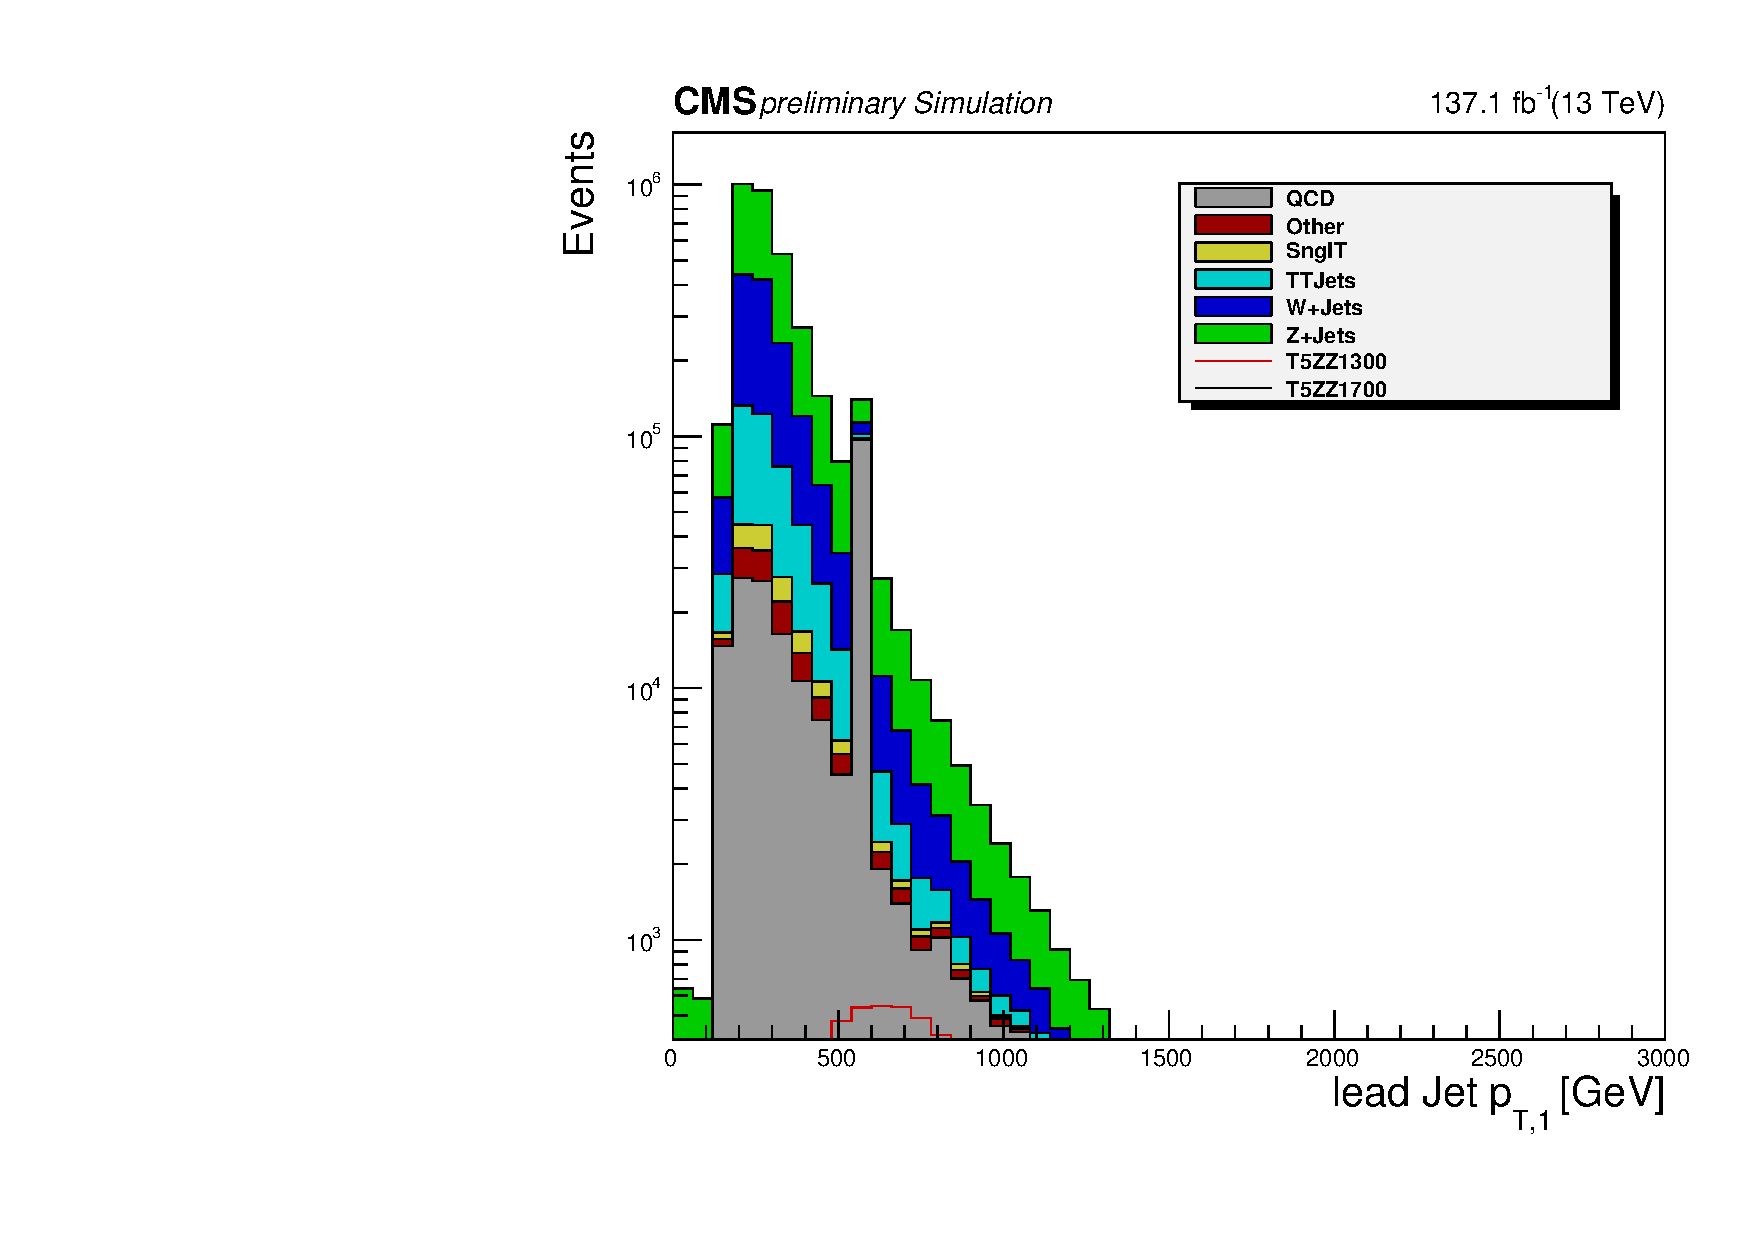
\includegraphics[width=0.48\linewidth]{plots/event-selection/2017JetPt1scaled137_baseline.pdf}
  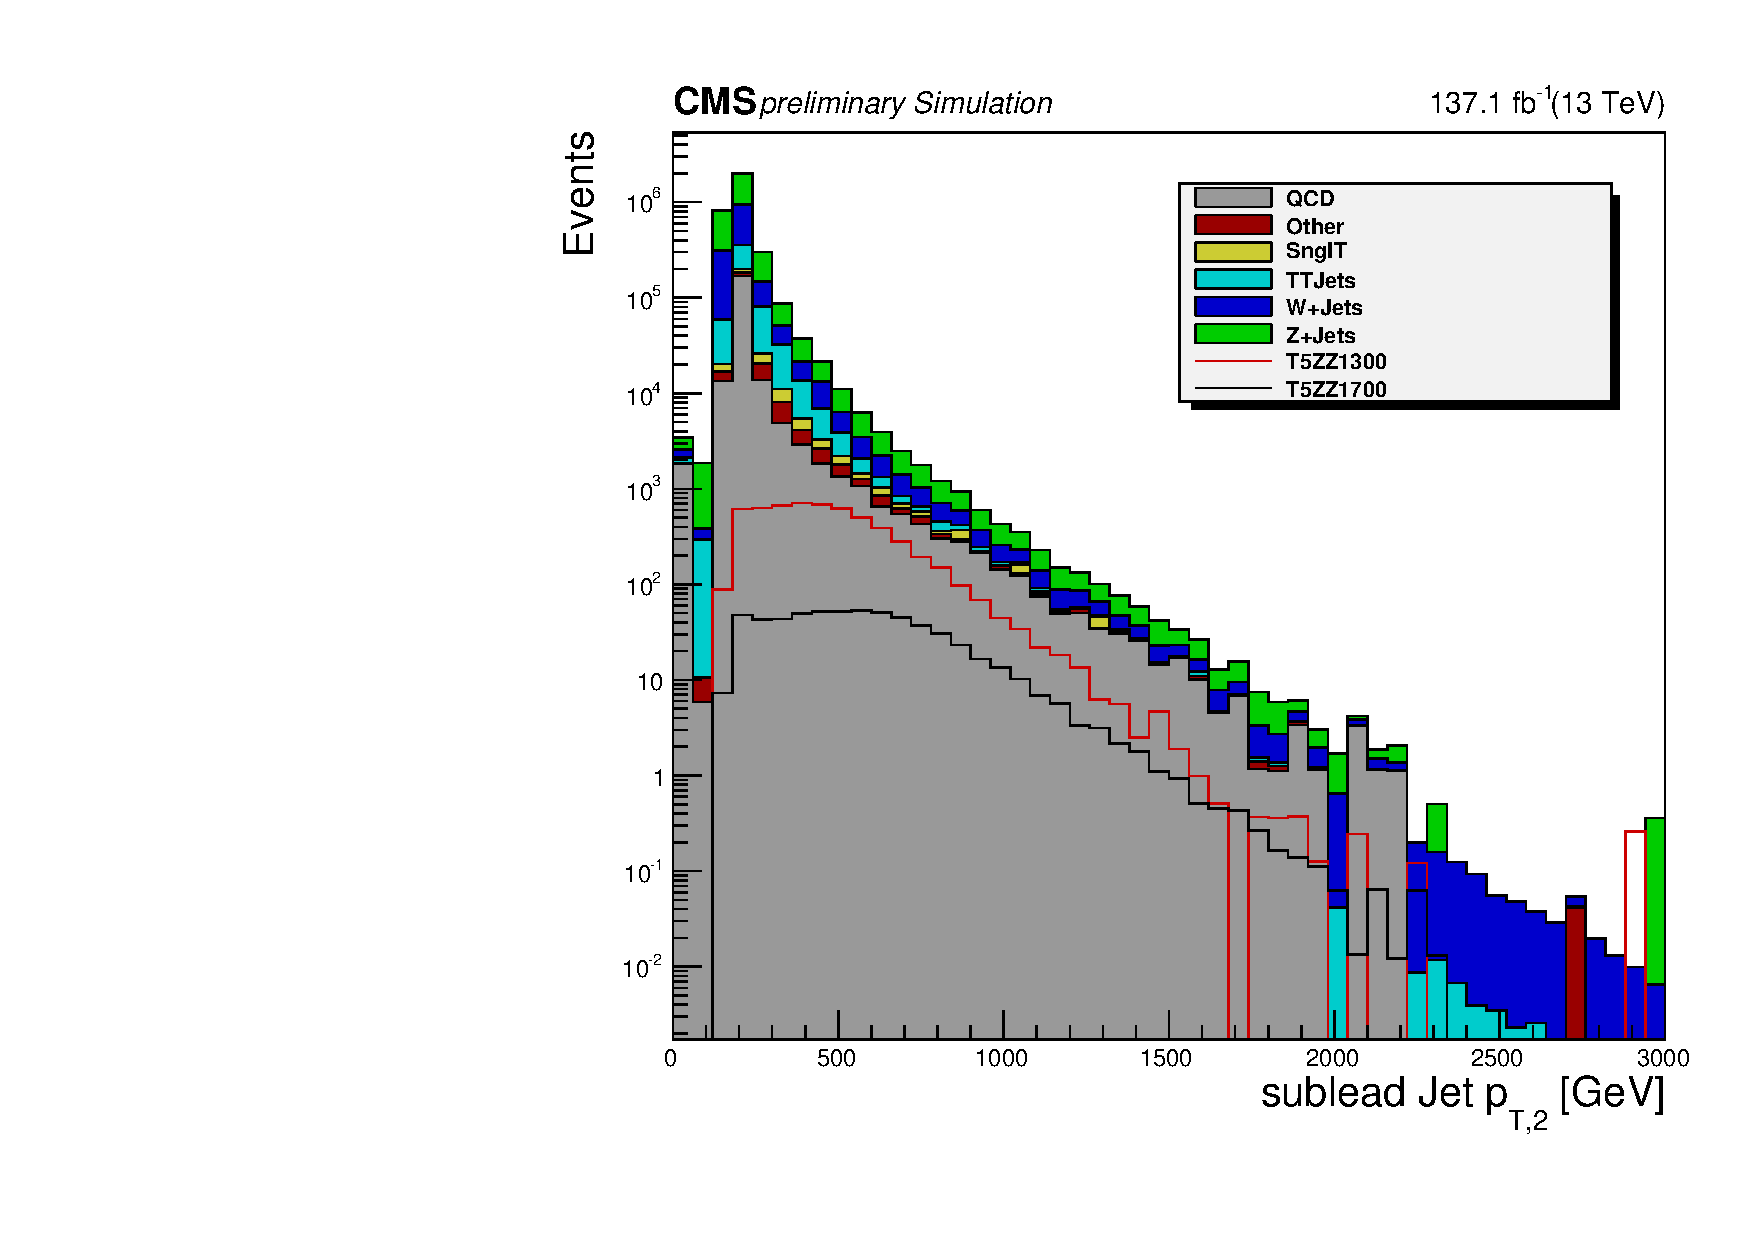
\includegraphics[width=0.48\linewidth]{plots/event-selection/2017JetPt2scaled137_baseline.pdf}\\[1mm]
  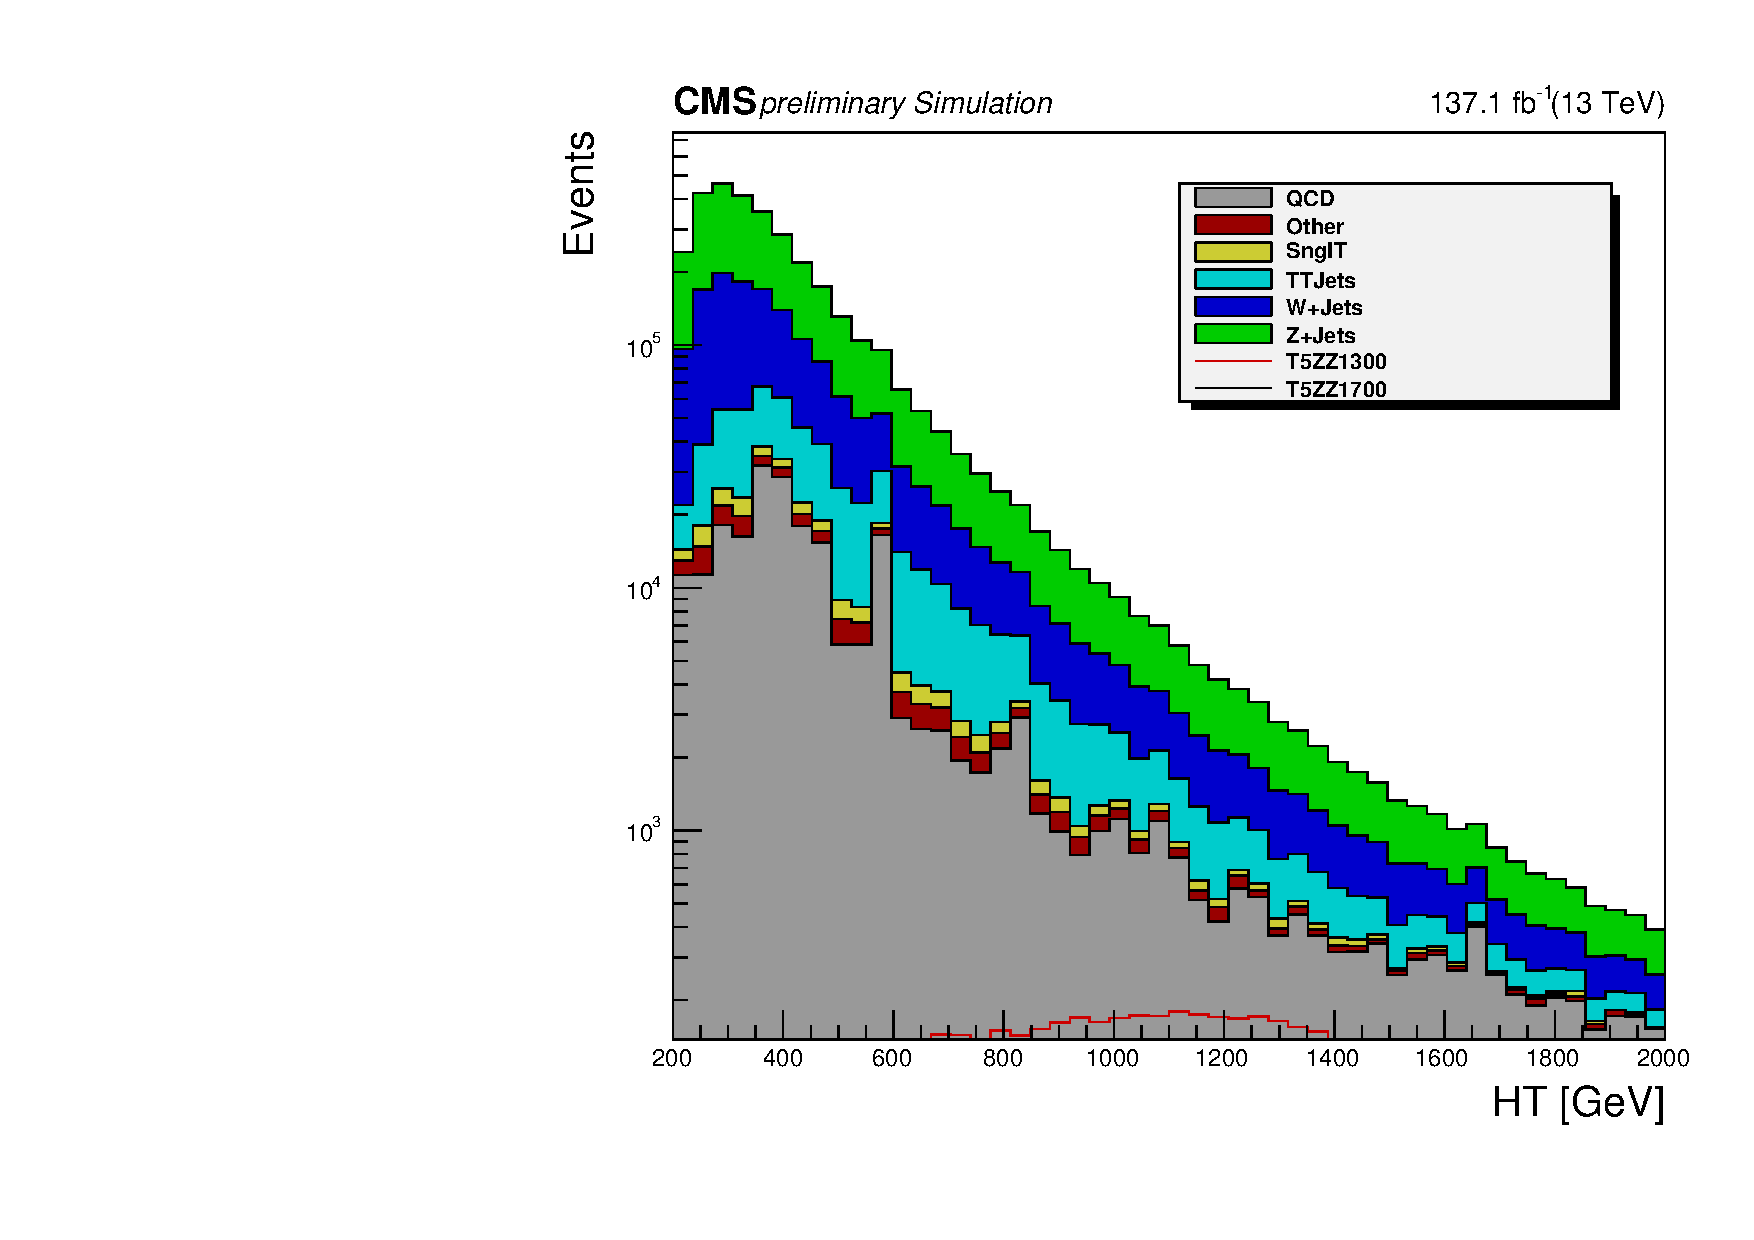
\includegraphics[width=0.48\linewidth]{plots/event-selection/2017HTscaled137_baseline.pdf}
  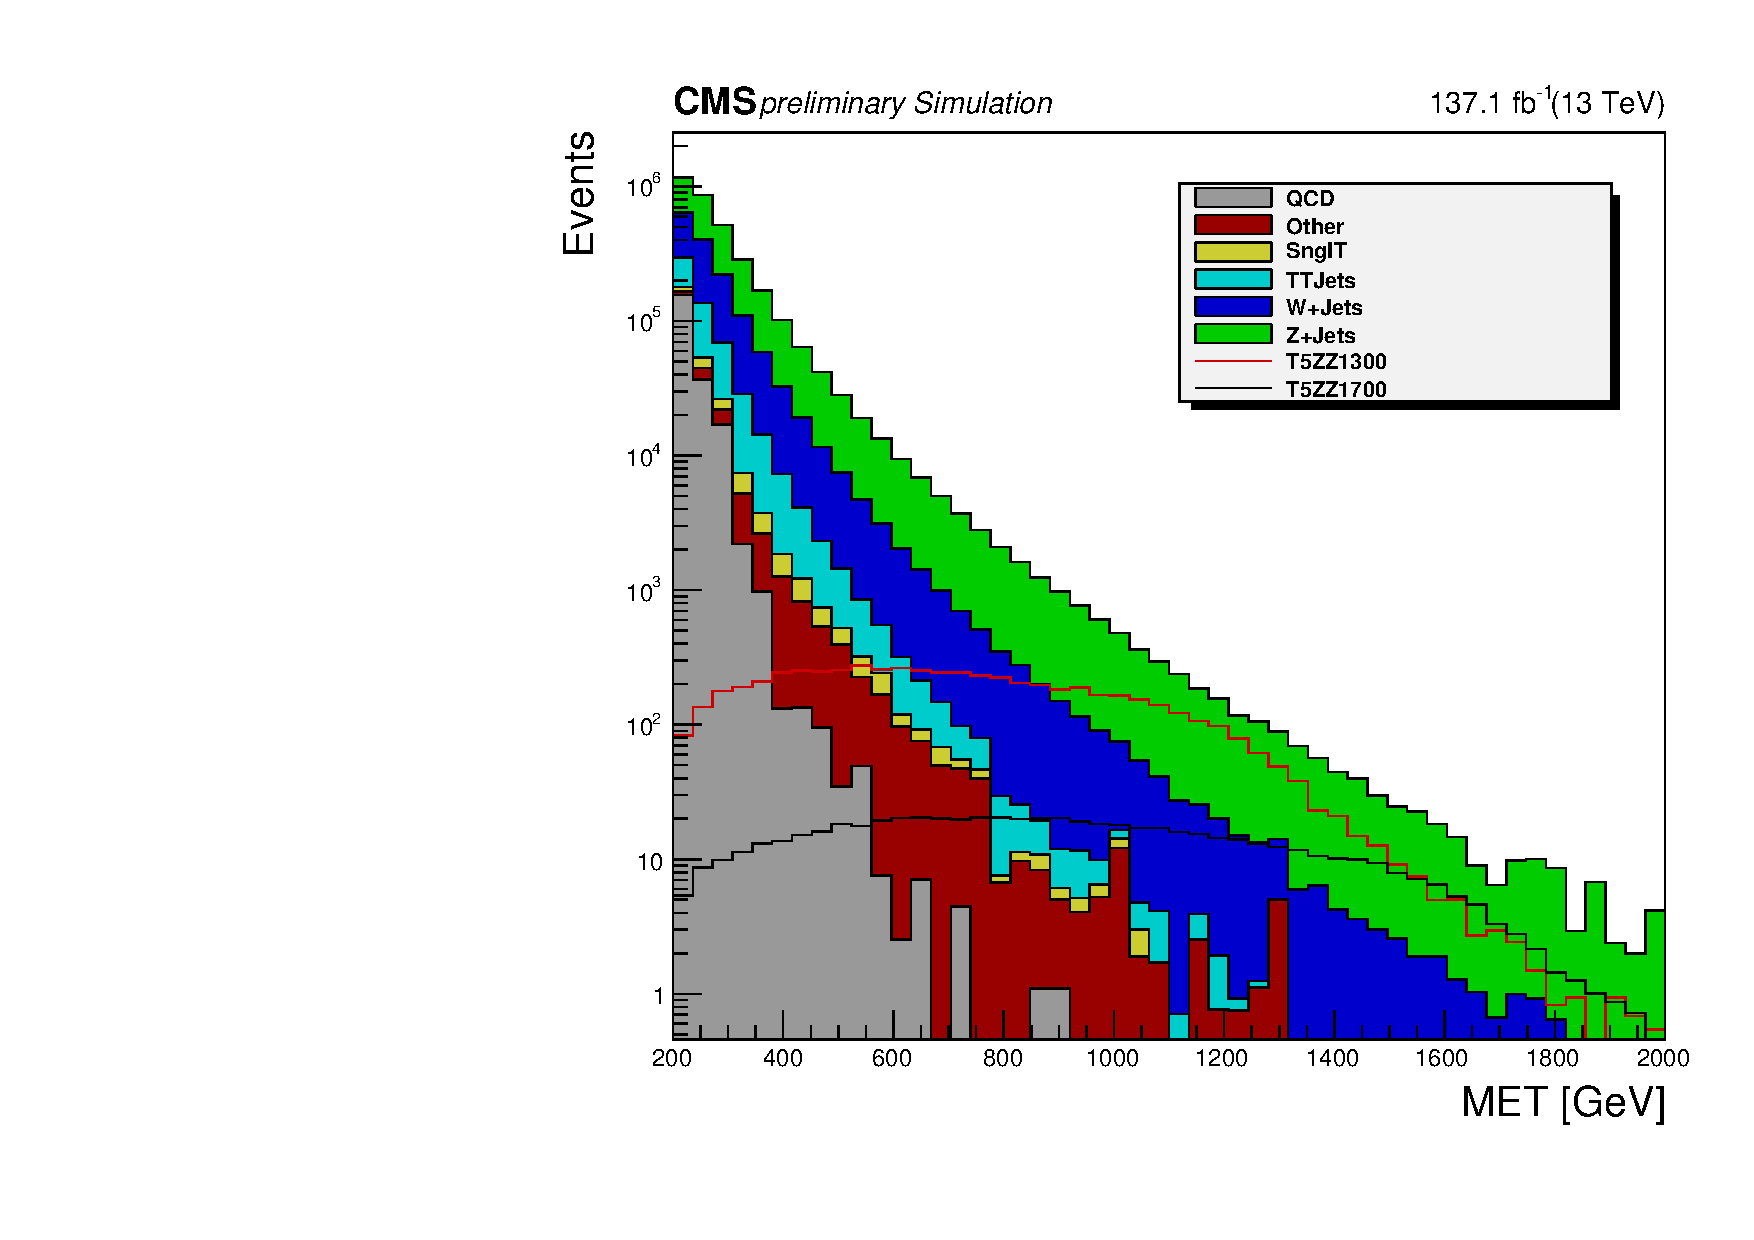
\includegraphics[width=0.48\linewidth]{plots/event-selection/2017METscaled137_baseline.pdf}\\[1mm]
 % \includegraphics[width=0.48\linewidth]{plots/event-selection/.pdf}
 % \includegraphics[width=0.48\linewidth]{plots/event-selection/.pdf}\\[1mm]
  \caption{
     Top: Jet \pt distributions after baseline selection except \HT,\MET, $\delta$R, jet mass and \pt requirements.
     Bottom:  \HT(left) and \MET(right) distributions after  baseline selection except \HT,\MET, $\delta$R, jet mass and \pt requirements.
  }
  \label{fig:cutFlow}
\end{figure}

\begin{figure}[htbp!]
  \centering
  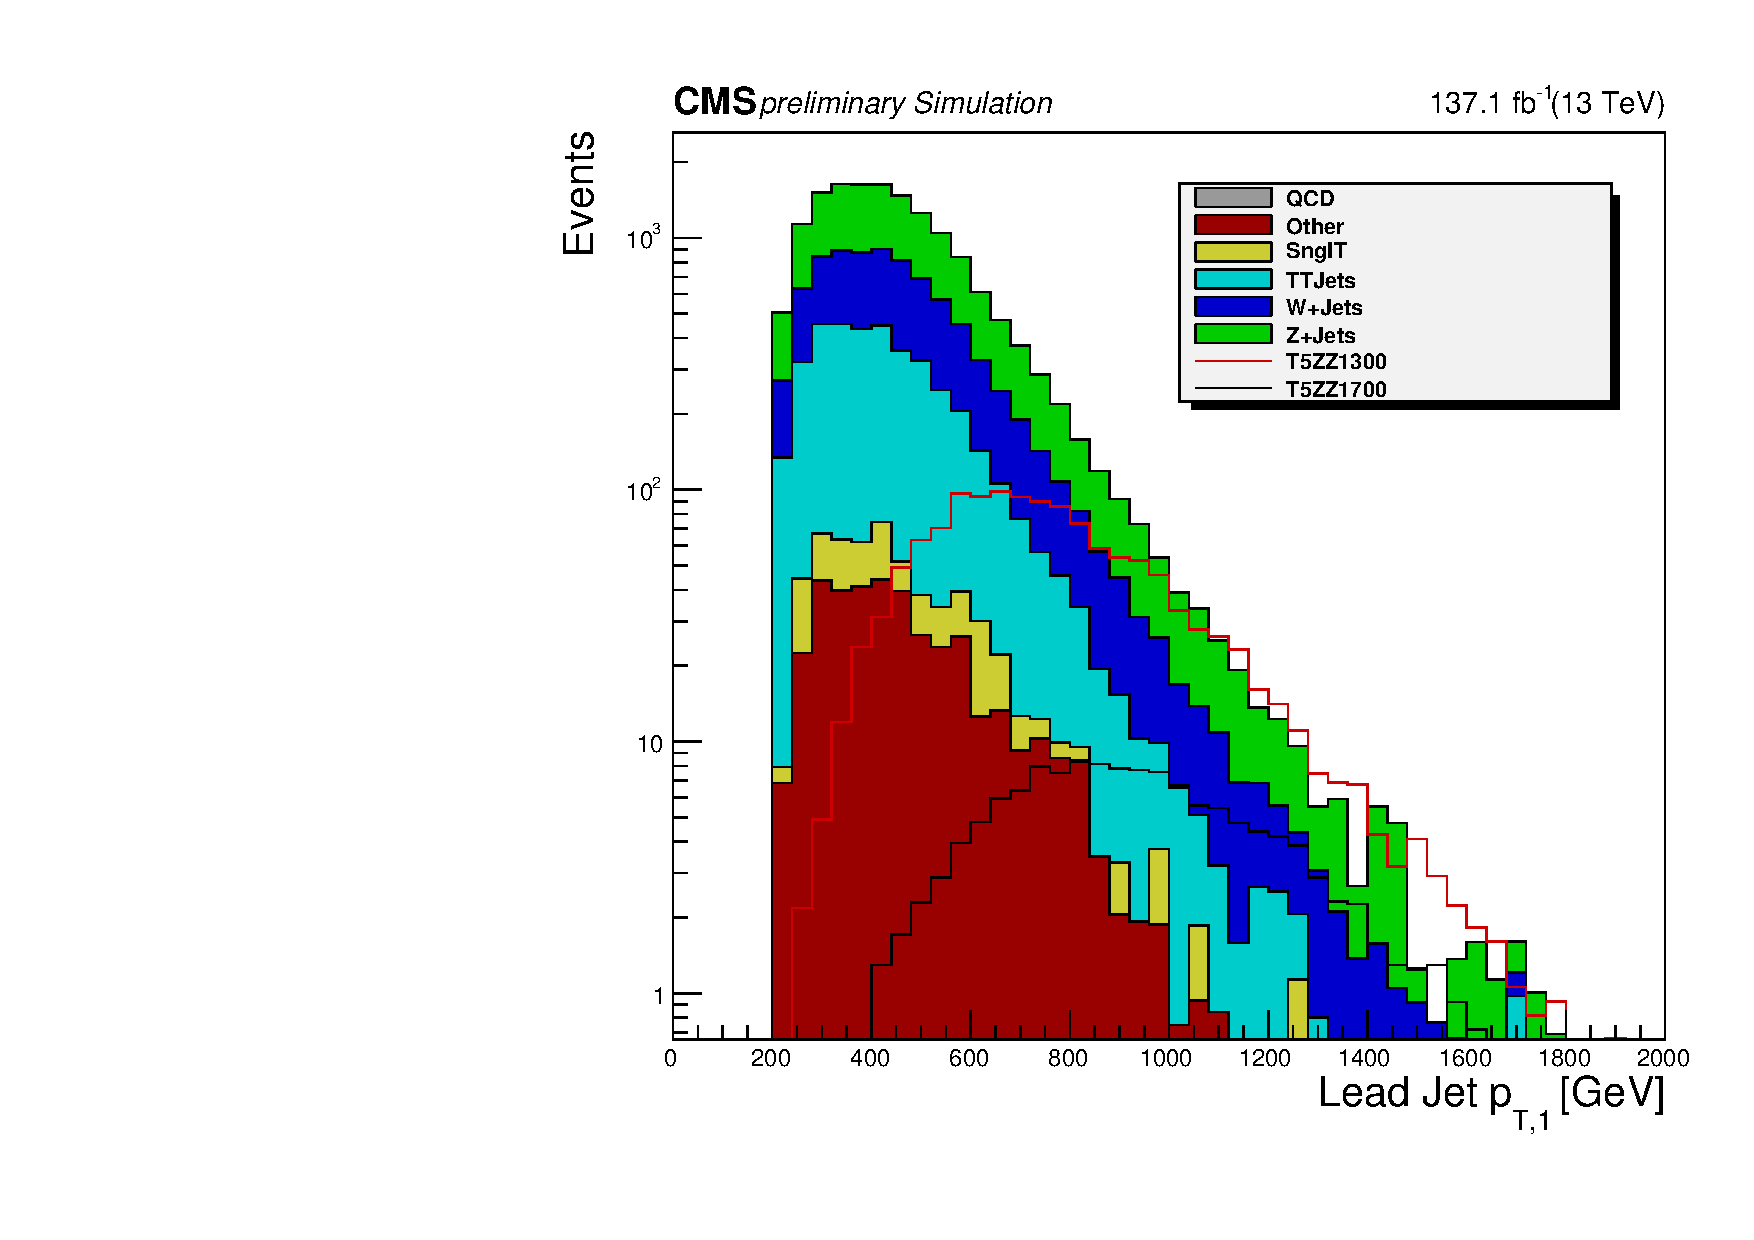
\includegraphics[width=0.48\linewidth]{plots/event-selection/JetPt1scaled137_selection.pdf}
  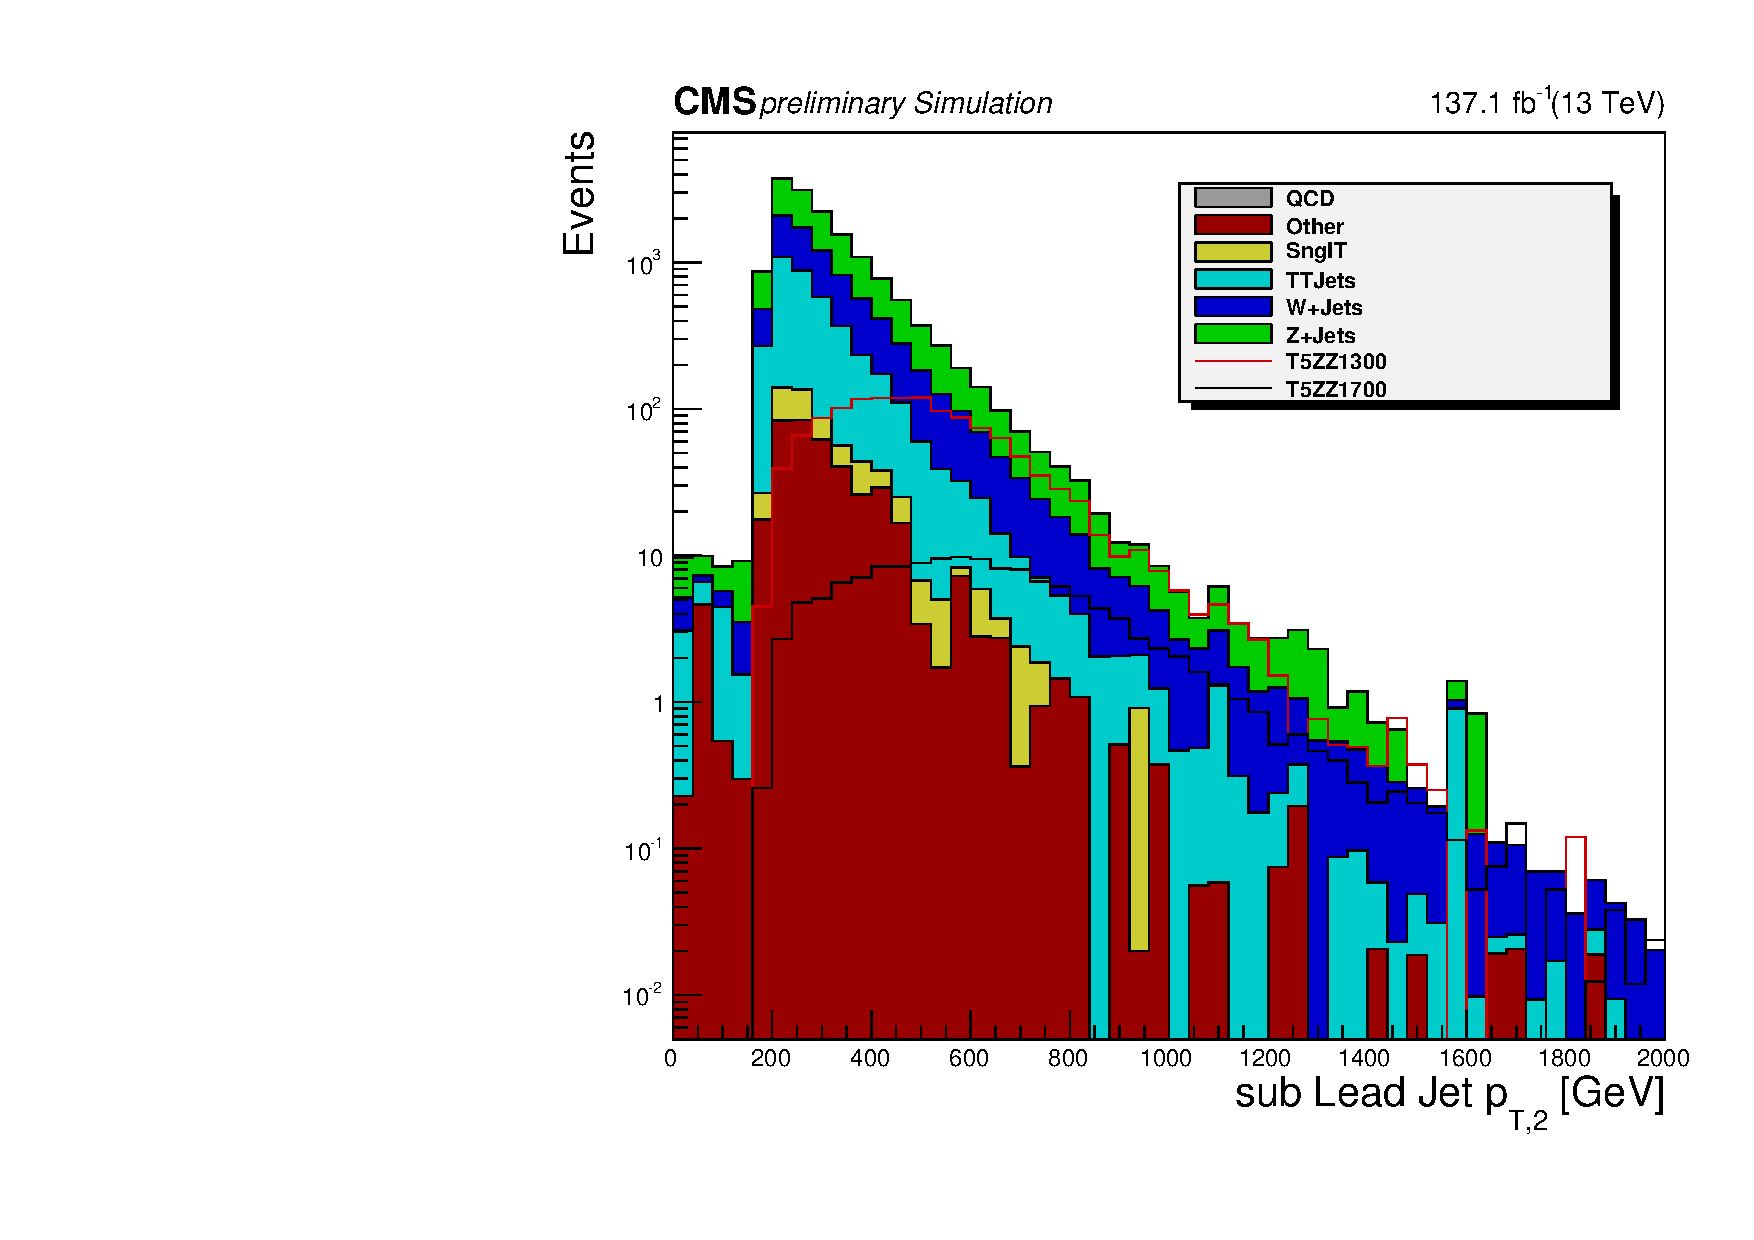
\includegraphics[width=0.48\linewidth]{plots/event-selection/JetPt2scaled137_selection.pdf}\\[1mm]
  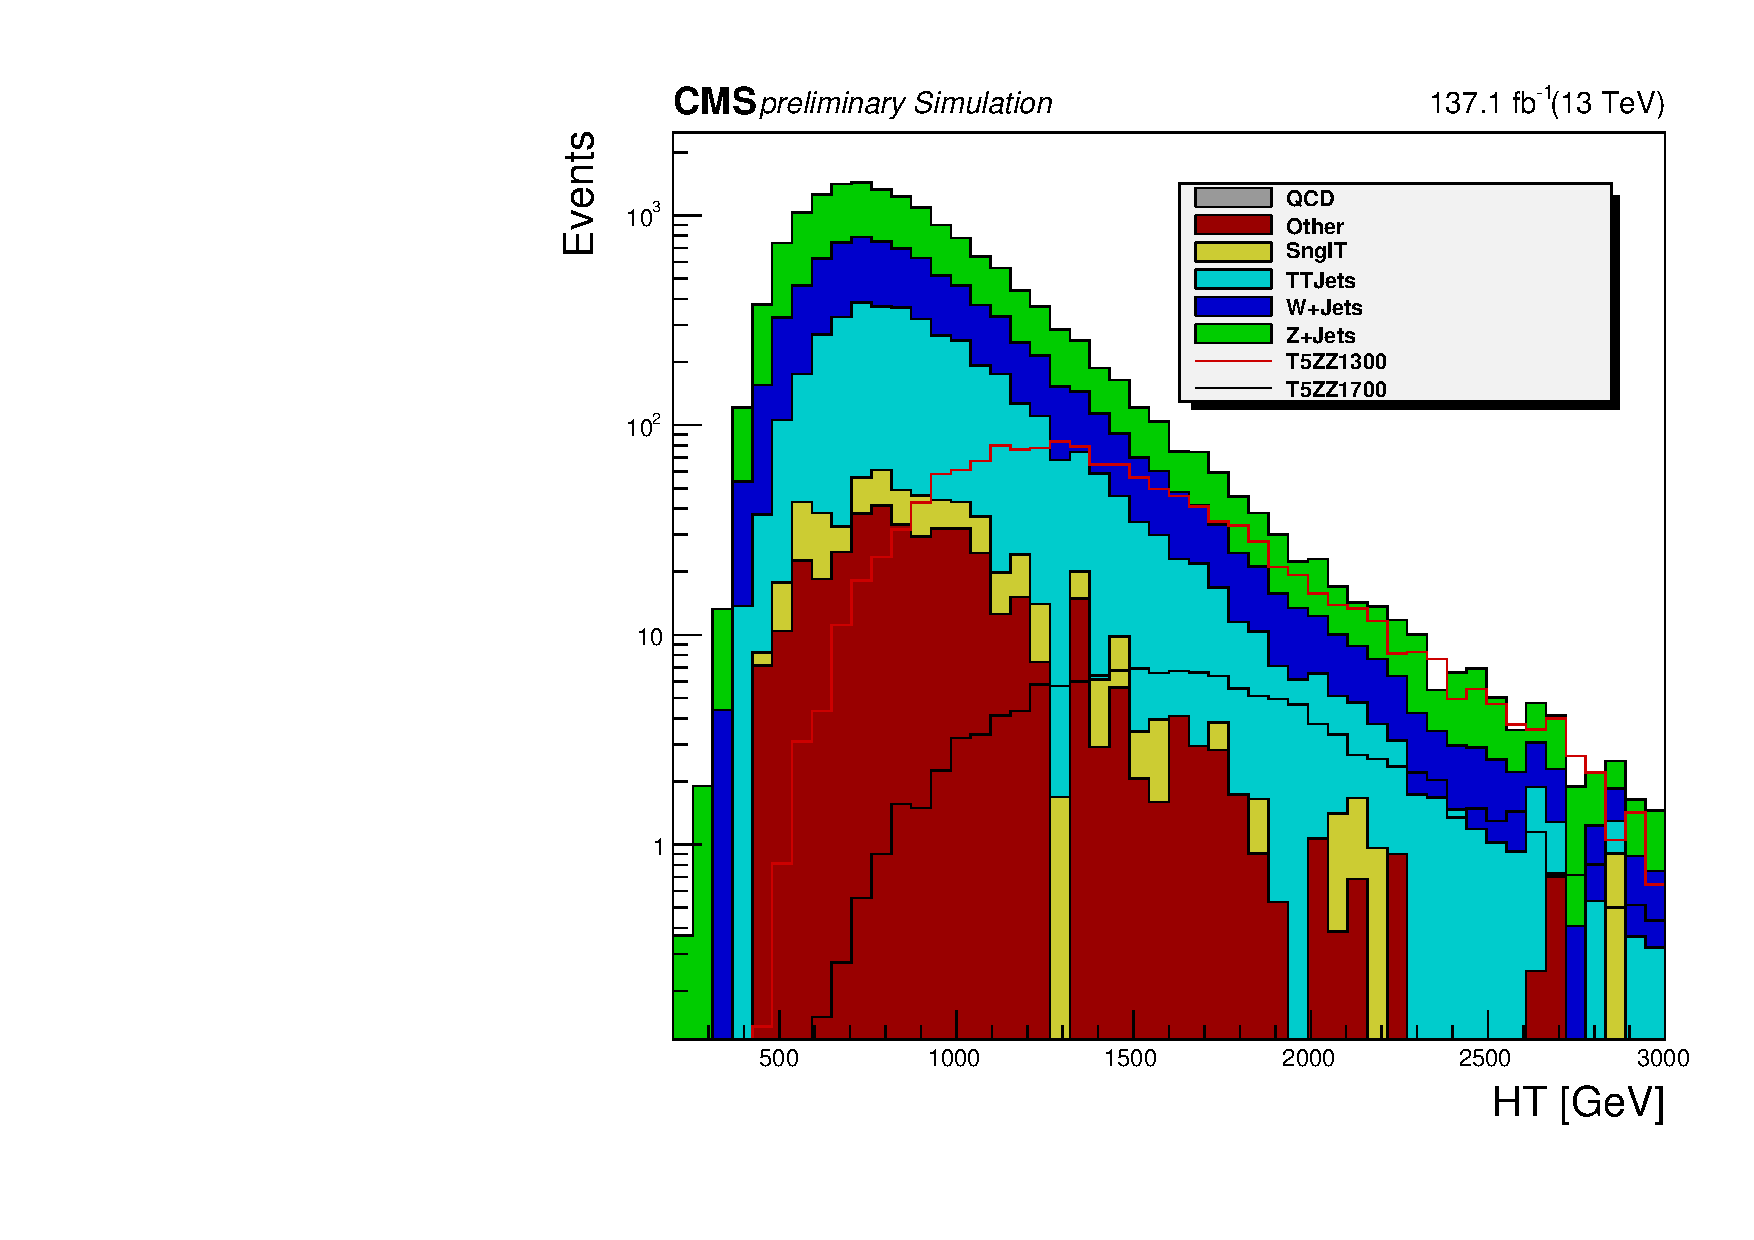
\includegraphics[width=0.48\linewidth]{plots/event-selection/HTscaled137_selection.pdf}
  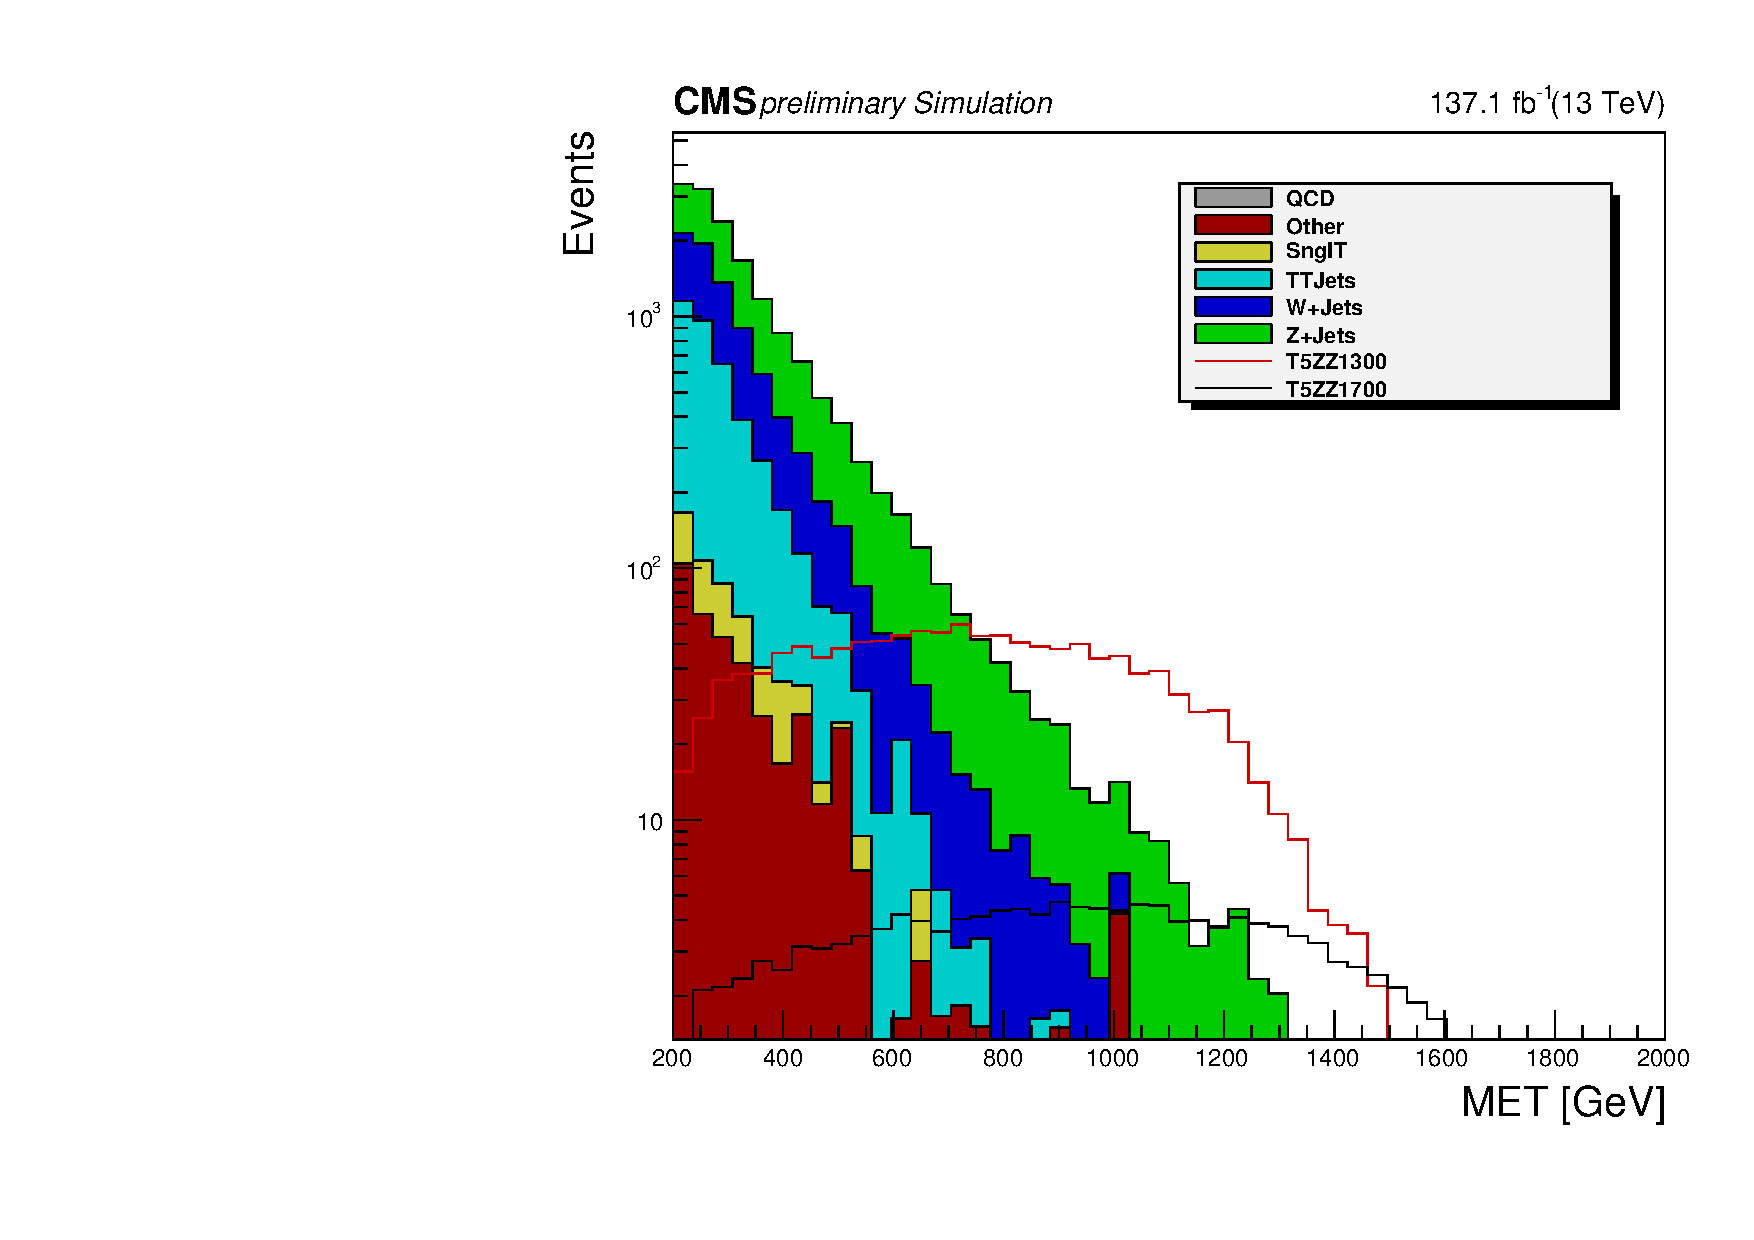
\includegraphics[width=0.48\linewidth]{plots/event-selection/METscaled137_selection.pdf}\\[1mm]
  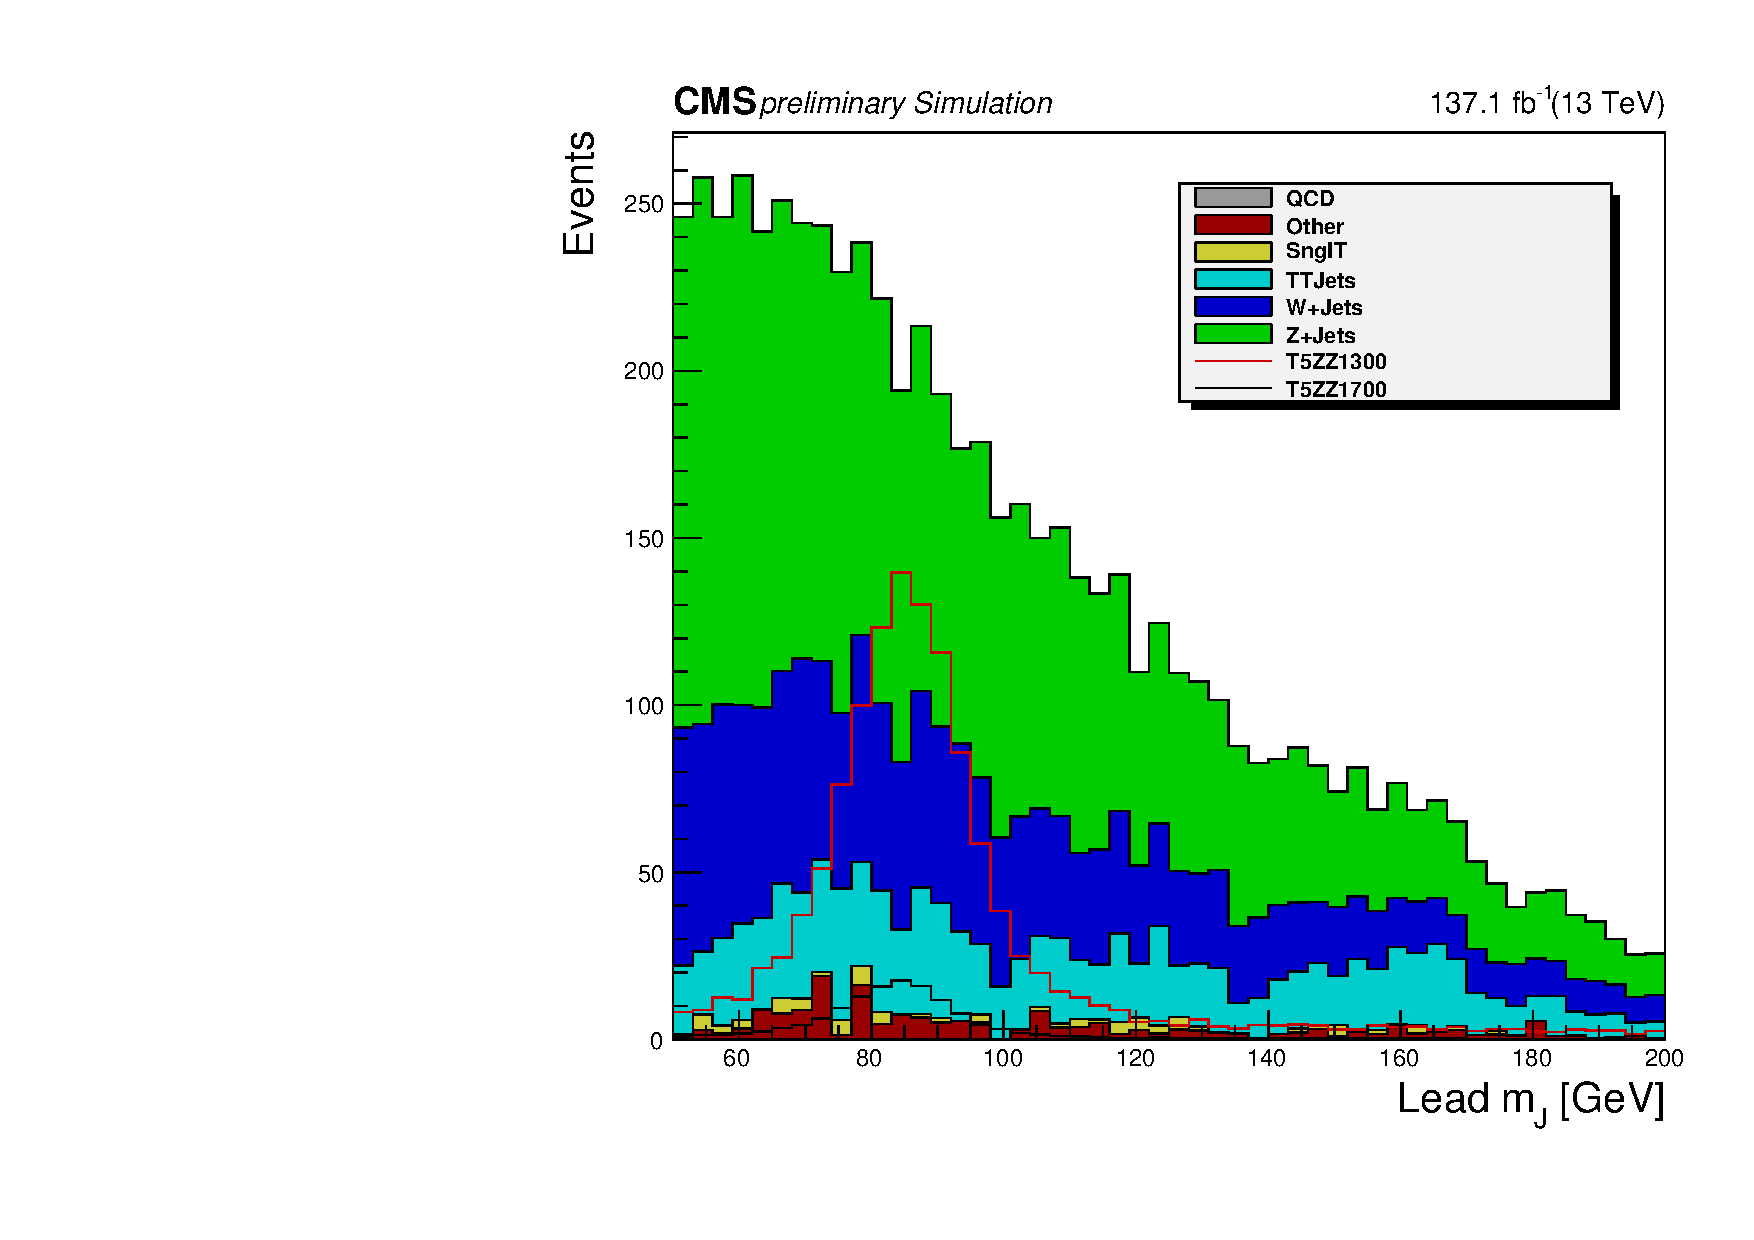
\includegraphics[width=0.48\linewidth]{plots/event-selection/PrunedMass1scaled137allselection.pdf}
  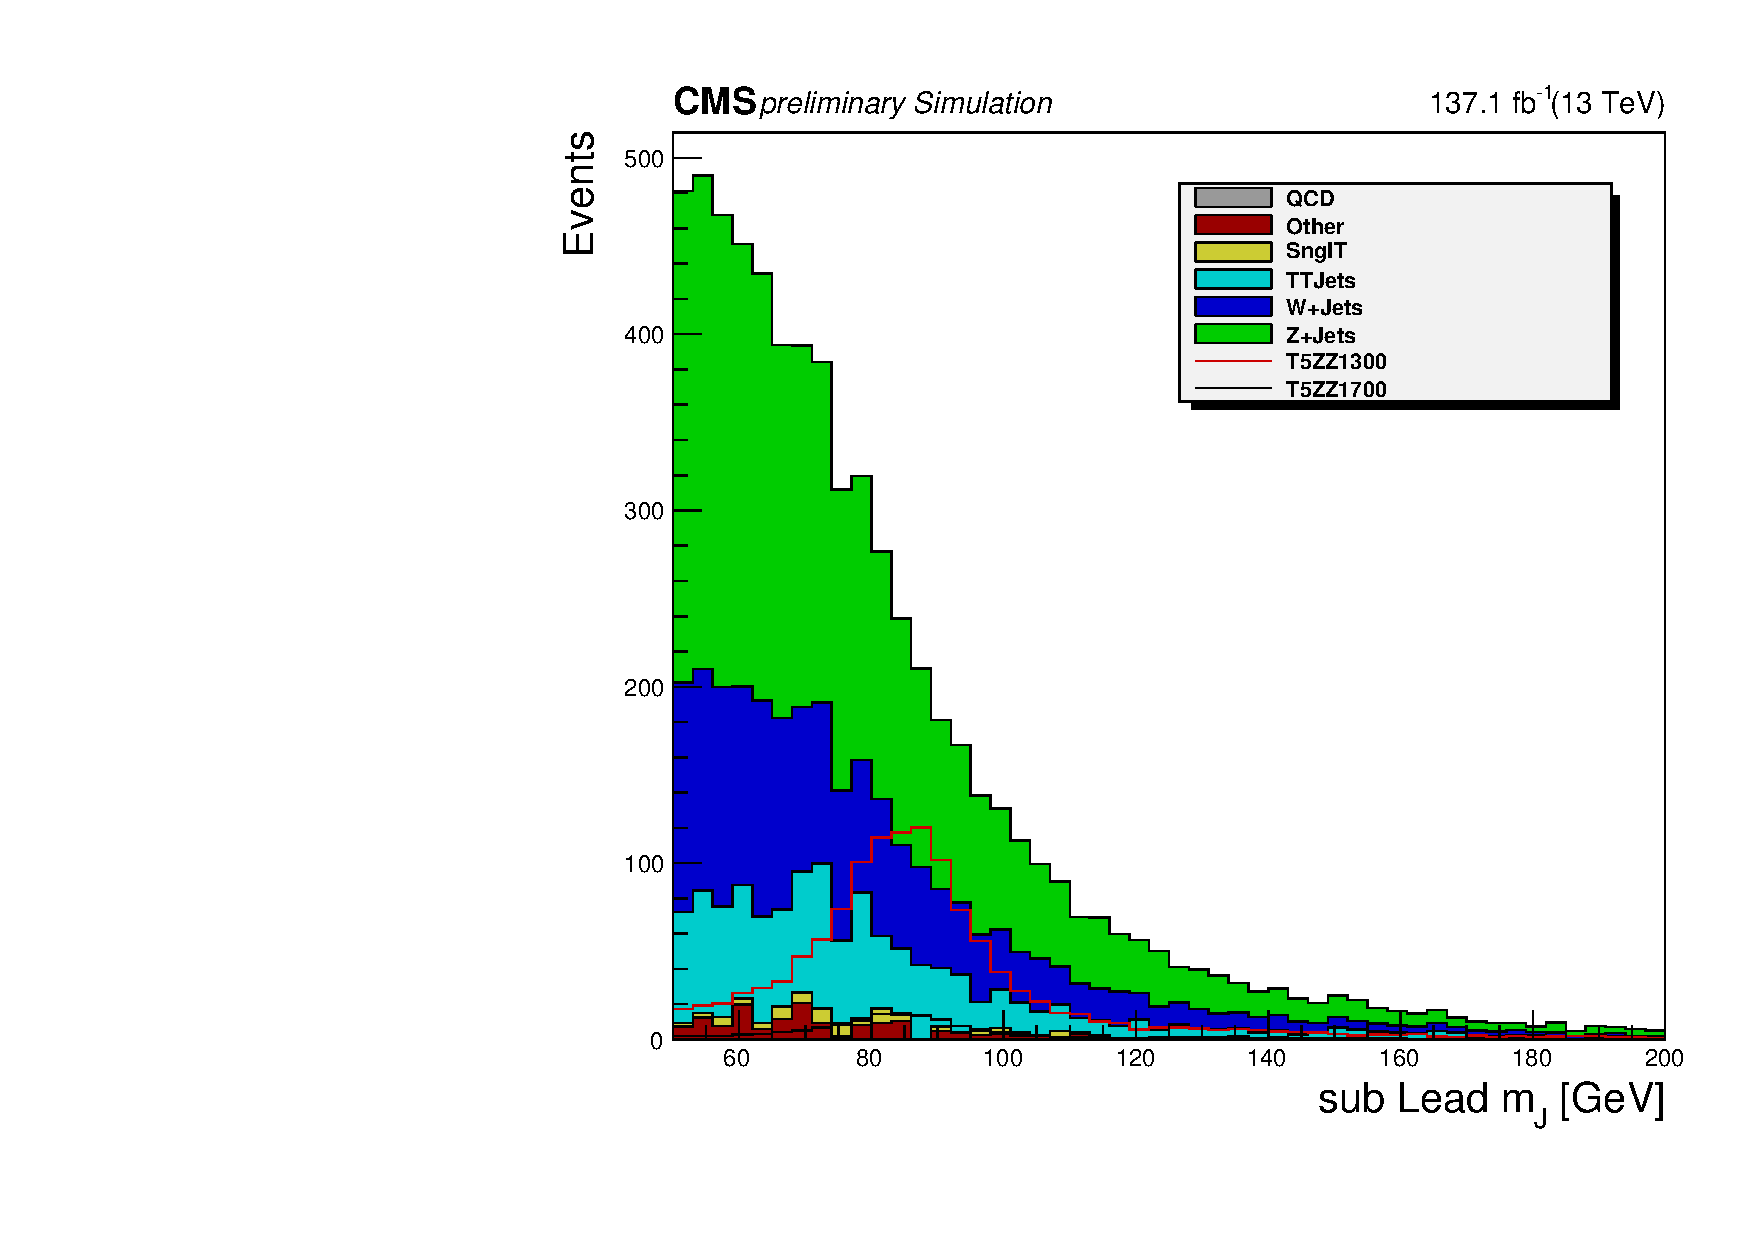
\includegraphics[width=0.48\linewidth]{plots/event-selection/PrunedMass2scaled137allselection.pdf}\\[1mm]
  \caption{
     Top: Jet \pt distributions after baseline selection except \HT,\MET and \pt requirements.
     Center:  \HT(left) and \MET(right) distributions after  baseline selection except \HT,\MET and \pt requirements.
     Bottom: Softdrop jet mass distributions after  baseline selection.
  }
  \label{fig:cutFlow2}
\end{figure}


\newpage
\begin{landscape}
 \begin{table}[htb!]
  \caption{
   Cut flow table for each of the main MC background samples and their sum. The table also includes the signal for two mass points of the 2Z final state. Cuts on the AK8 jets are applied to both the leading and subleading jets.
  }
  \begin{tabular}{|c|c|c|c|c|c|c|c|}
   \hline
	\hline
   Cut & Total Bkg. & $Z\rightarrow\nu\nu$ & $W\rightarrow\ell\nu$ & $t\overline{t}$ & QCD & T5HH1300 & T5HH1700  \\
	\hline
	\hline
	\multicolumn{8}{c}{Baseline SUSY Hadronic Skim: $\met>300\gev$, $HT>300\gev$, $\Delta\phi$ cuts, Lepton Veto, Isolated Track Veto}\\
   \hline
	Baseline SUSY Hadronic Skim &  439015 & 293825 & 118287 & 26121 & 780 & 1550  & 169 \\ \hline
	$\met>300\gev$ & 112300 & 69855 & 26868 & 14806 & 769 & 1525 & 159.4 \\ \hline
	$HT>500\gev$ & 46153 & 26409 & 10661 & 8627 & 455.8 &  1486 & 159.4 \\ \hline
	AK8 Lead Jet $\pt>300\gev$ &  42321  & 24672 & 9835 & 7502 & 310.1 & 1342  & 143.9 \\ \hline
	AK8 subLead Jet $\pt>200\gev$ & 29577  & 17428 & 6935.5  & 4940.7 &  272.5& 1183  & 128 \\ \hline
	AK8 Jet Mass in $[50,200]\gev$ & 6107.8 & 2964.8 & 1292.1 & 1789.1 &61.7 &   785 &  86   \\ \hline
	$\Delta$ R $>$ 0.8 for sublead AK8 Jet &2478 & 1400 & 668.3 & 378.7 &31 & 402 & 44  \\ \hline
	AK8 Jet Mass in $[70,100]\gev$ &  284.1 & 161 & 78.8 & 42.8 & 1.37 & 229 & 28\\ \hline
   \hline
   \hline
   \end{tabular}
   \label{tab:Cutflow}
  \end{table}
\end{landscape}

\subsection{Signal Regions}

\begin{figure}[htbp!]
  \begin{center}
    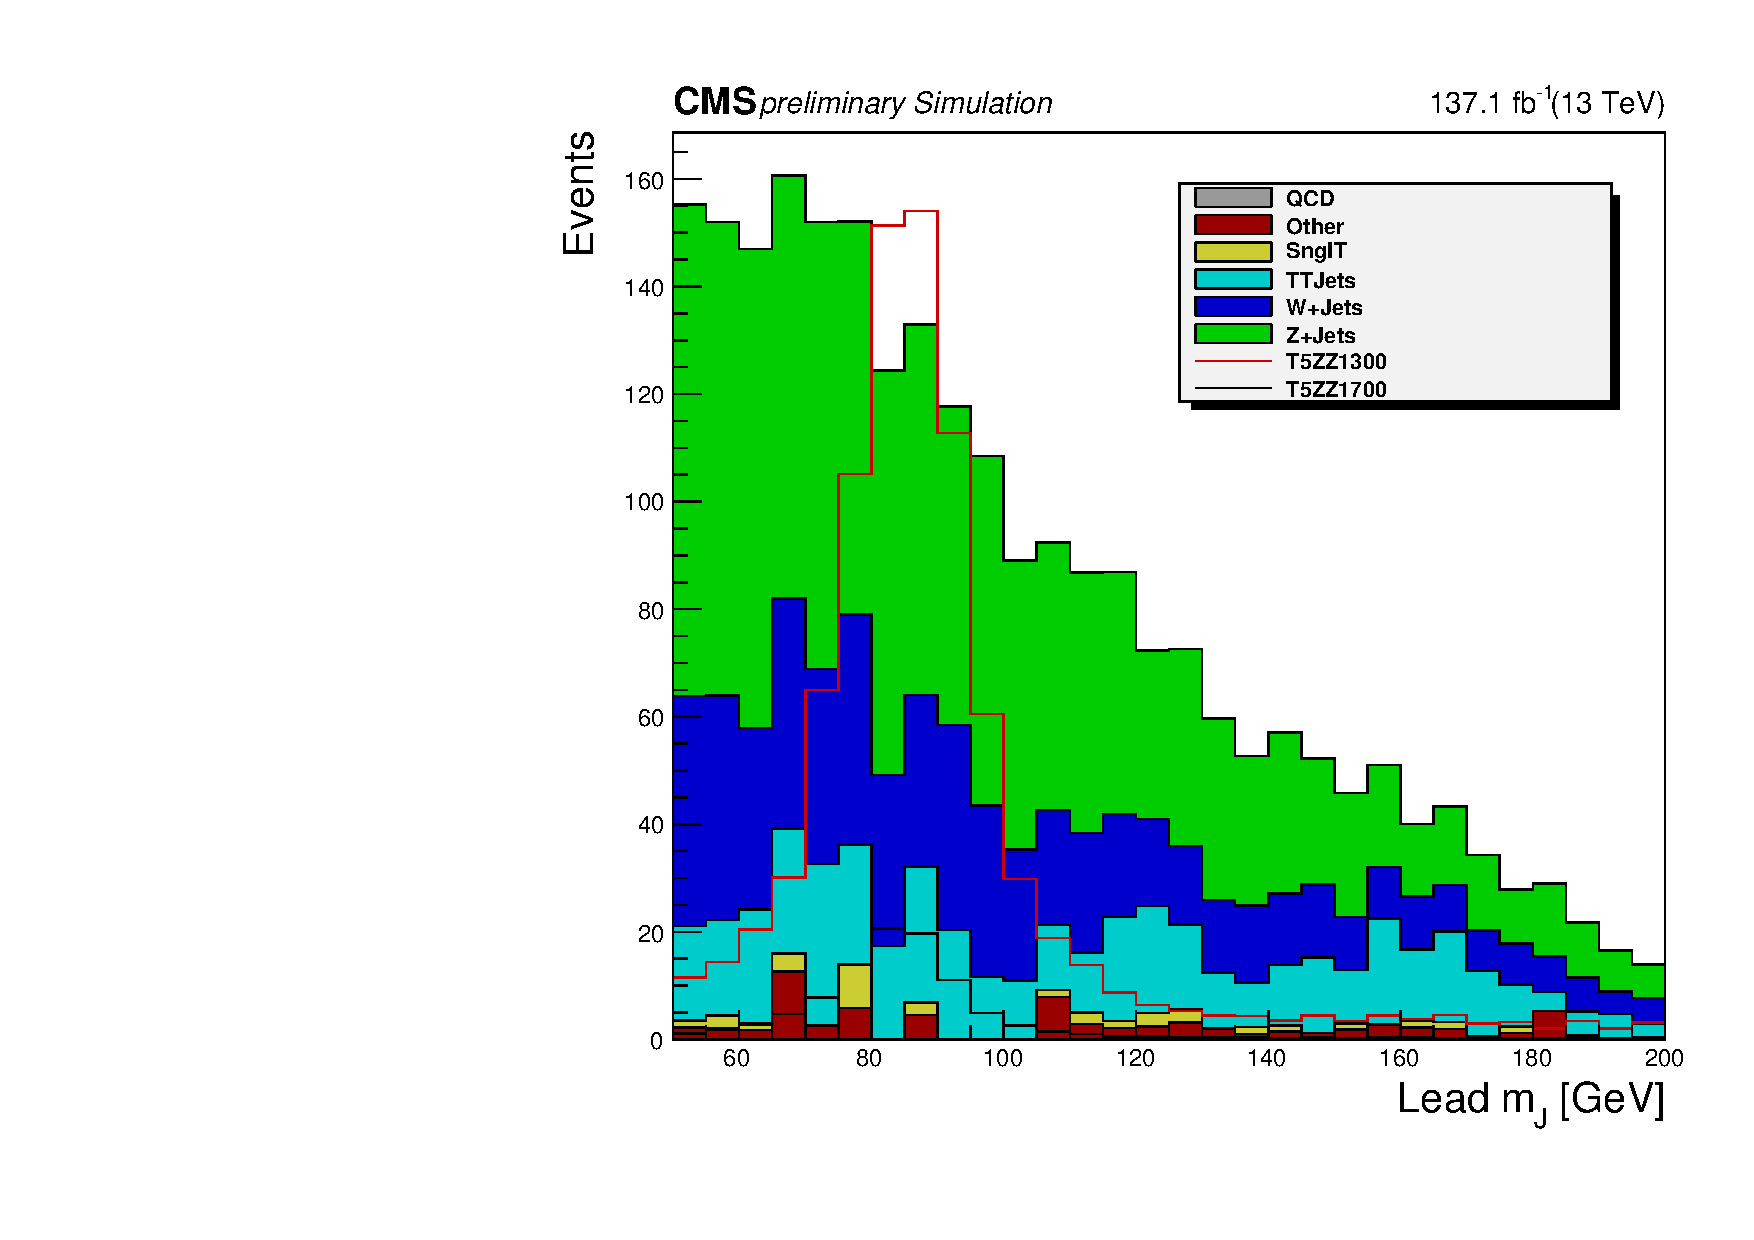
\includegraphics[trim={5px 5px 5px 5px},clip,width=0.48\linewidth]{plots/event-selection/PrunedMass1scaled137_fitting.pdf}
    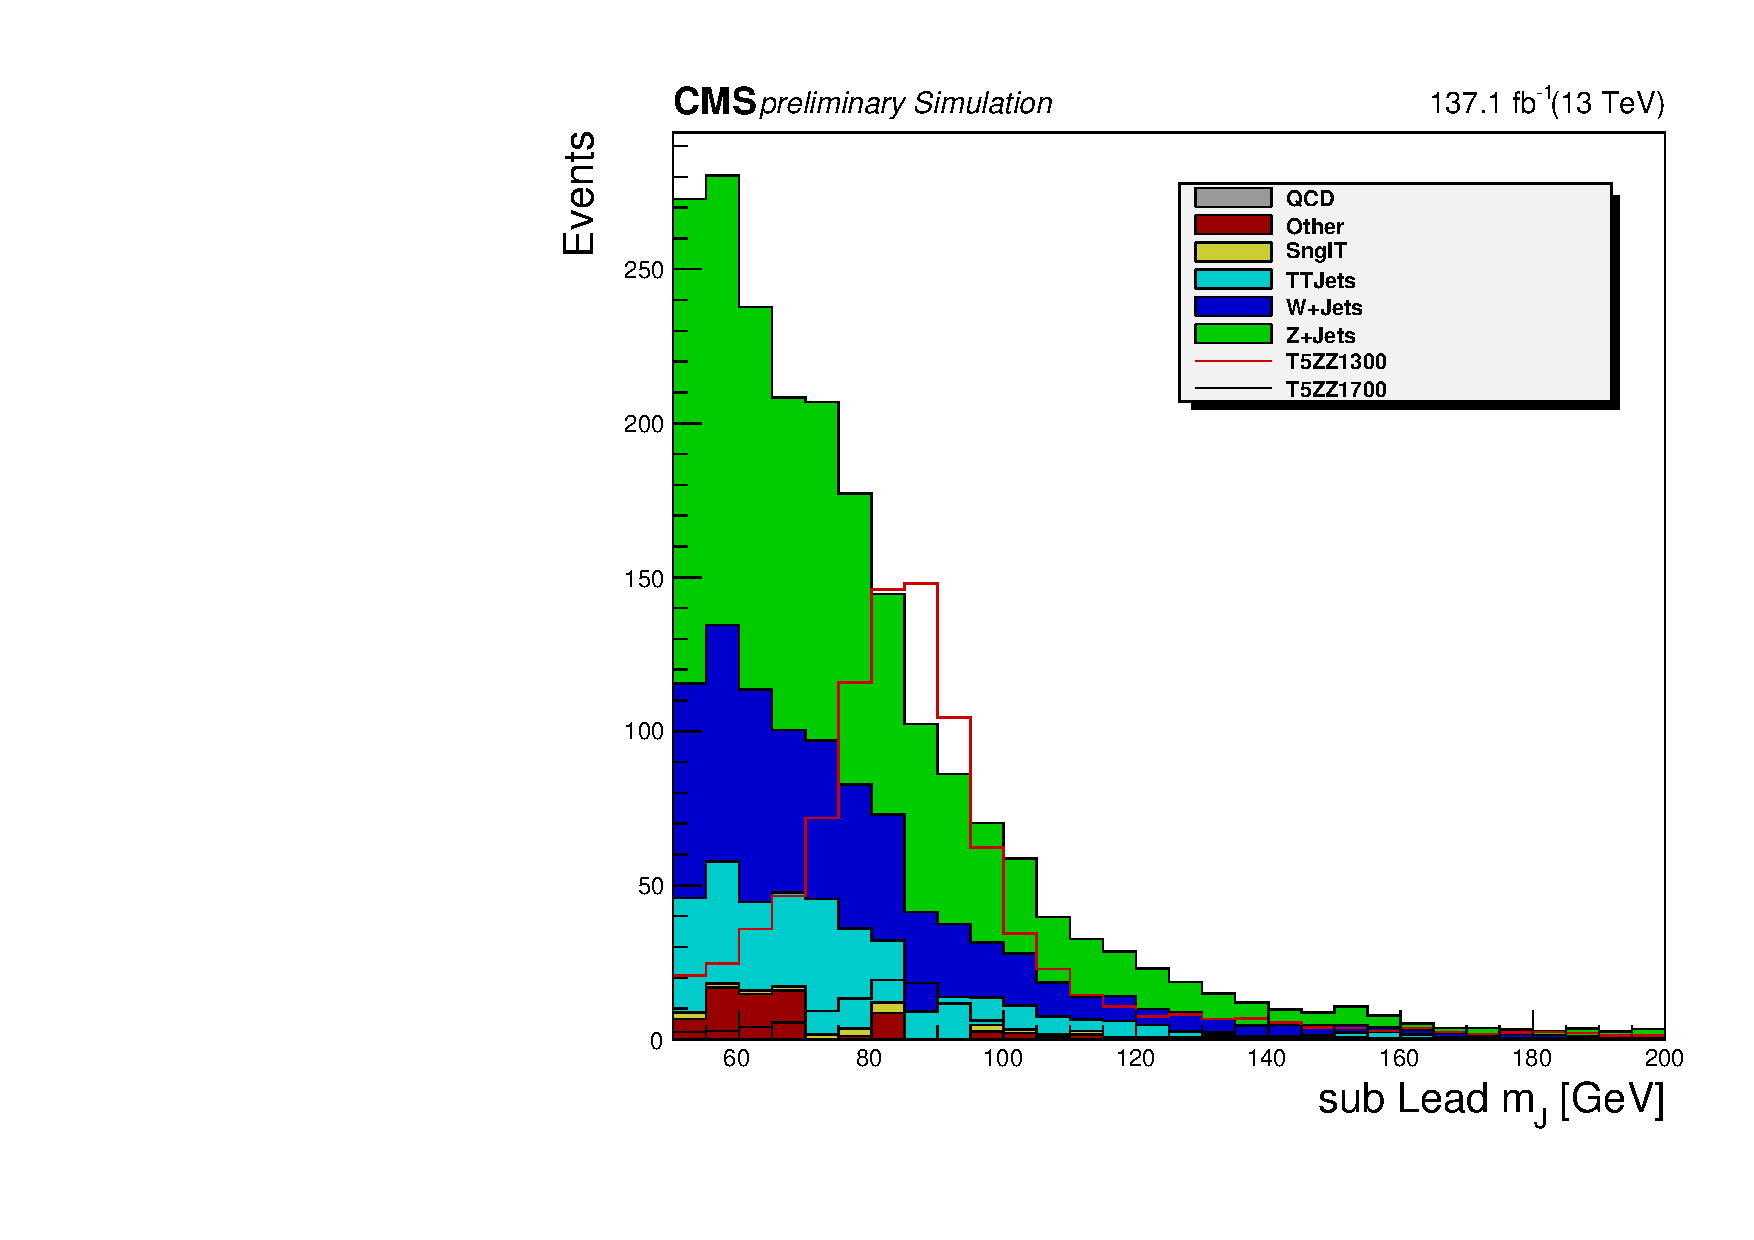
\includegraphics[trim={5px 5px 5px 5px},clip,width=0.48\linewidth]{plots/event-selection/PrunedMass2scaled137_fitting.pdf}
    \caption{
      Distribution of the leading (left) and subleading (right) AK8 pruned-jet mass after the baseline selection, for leading jet baseline selections are all but lead jet mass[50,200] and for sublead jet vice-versa.
    }
    \label{fig:JetMass_baseline}
  \end{center}
\end{figure}


\subsection{Control Regions}


\def \bkgestimationPlotsDir {plots/bkgestimation/}

\section{Background Estimation Method}
\label{sec:bkgest}


%Note, this is equivalent to saying that the ratio of yeilds in the
%tagged region and the yields in the anti-tagged region, R$_{pass/fail}$, is independent of the mass. 
%\begin{figure}[htbp!]

%  \begin{center}
%    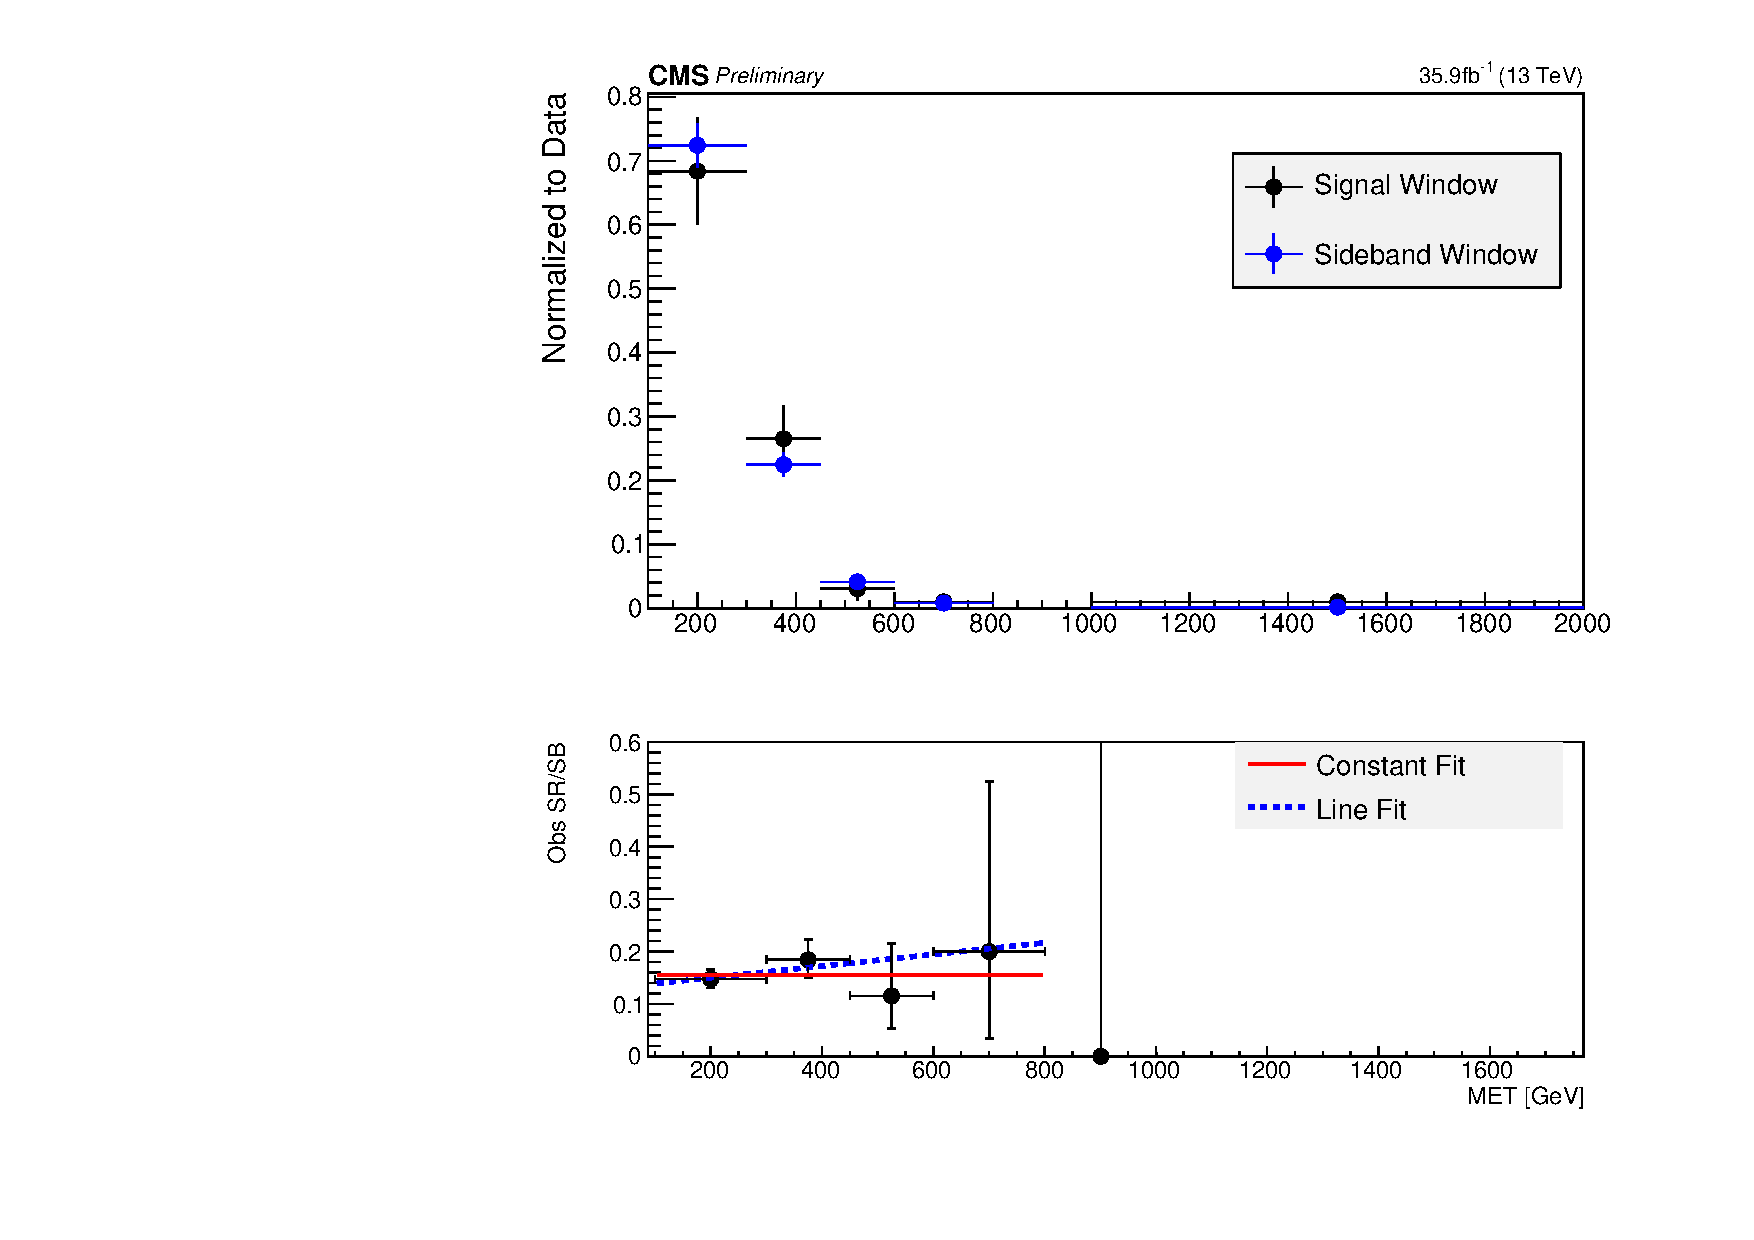
\includegraphics[trim={5px 5px 5px 5px},clip,width=0.6\linewidth]{plots/bkgestimation/Data2016SingleLepton.pdf}
%    \caption{ 2016 Data validation of SR and SB 
%    }
%    \label{fig:Data2016SingleLepton}
%  \end{center}
%\end{figure} 


\begin{figure}[htbp!]
  \begin{center}
    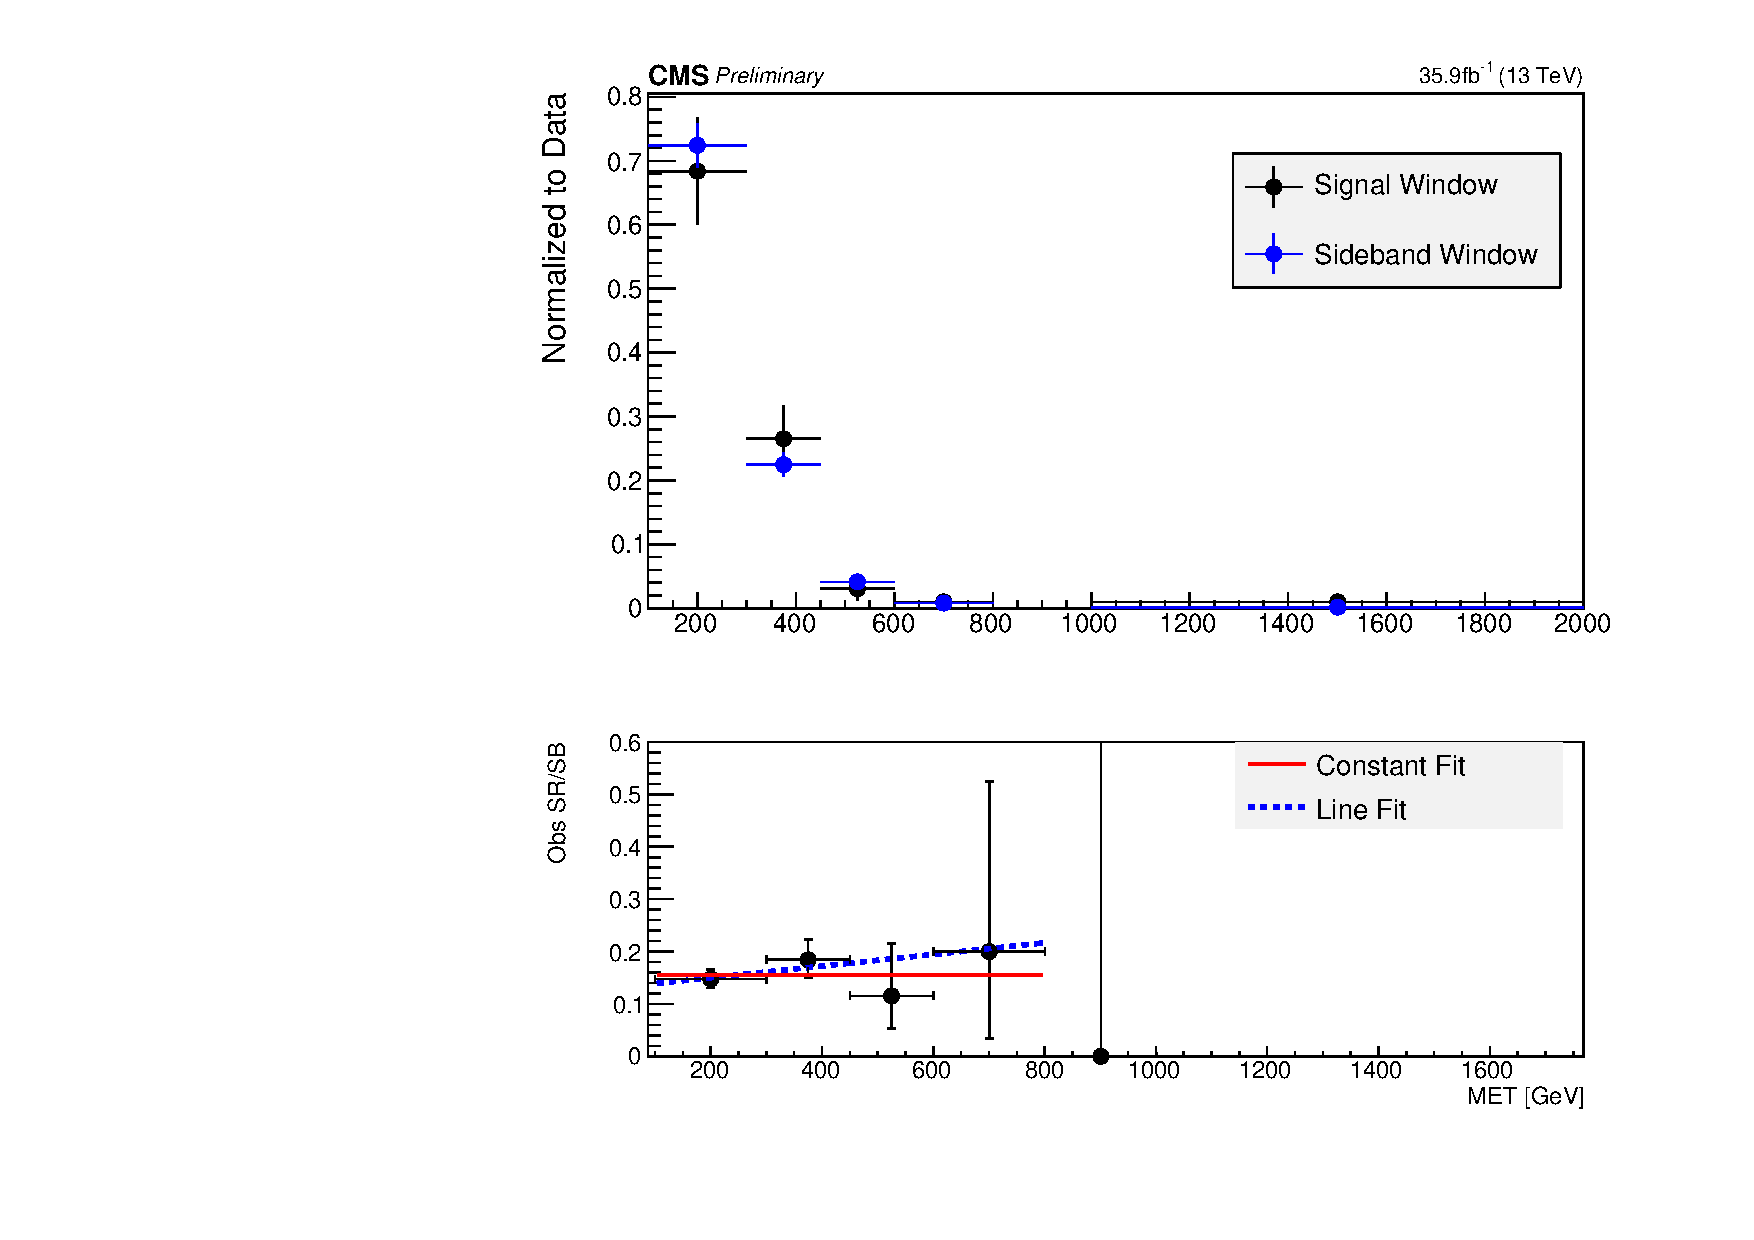
\includegraphics[trim={5px 5px 5px 5px},clip,width=0.48\linewidth]{plots/bkgestimation/Data2016SingleLepton.pdf}\\
    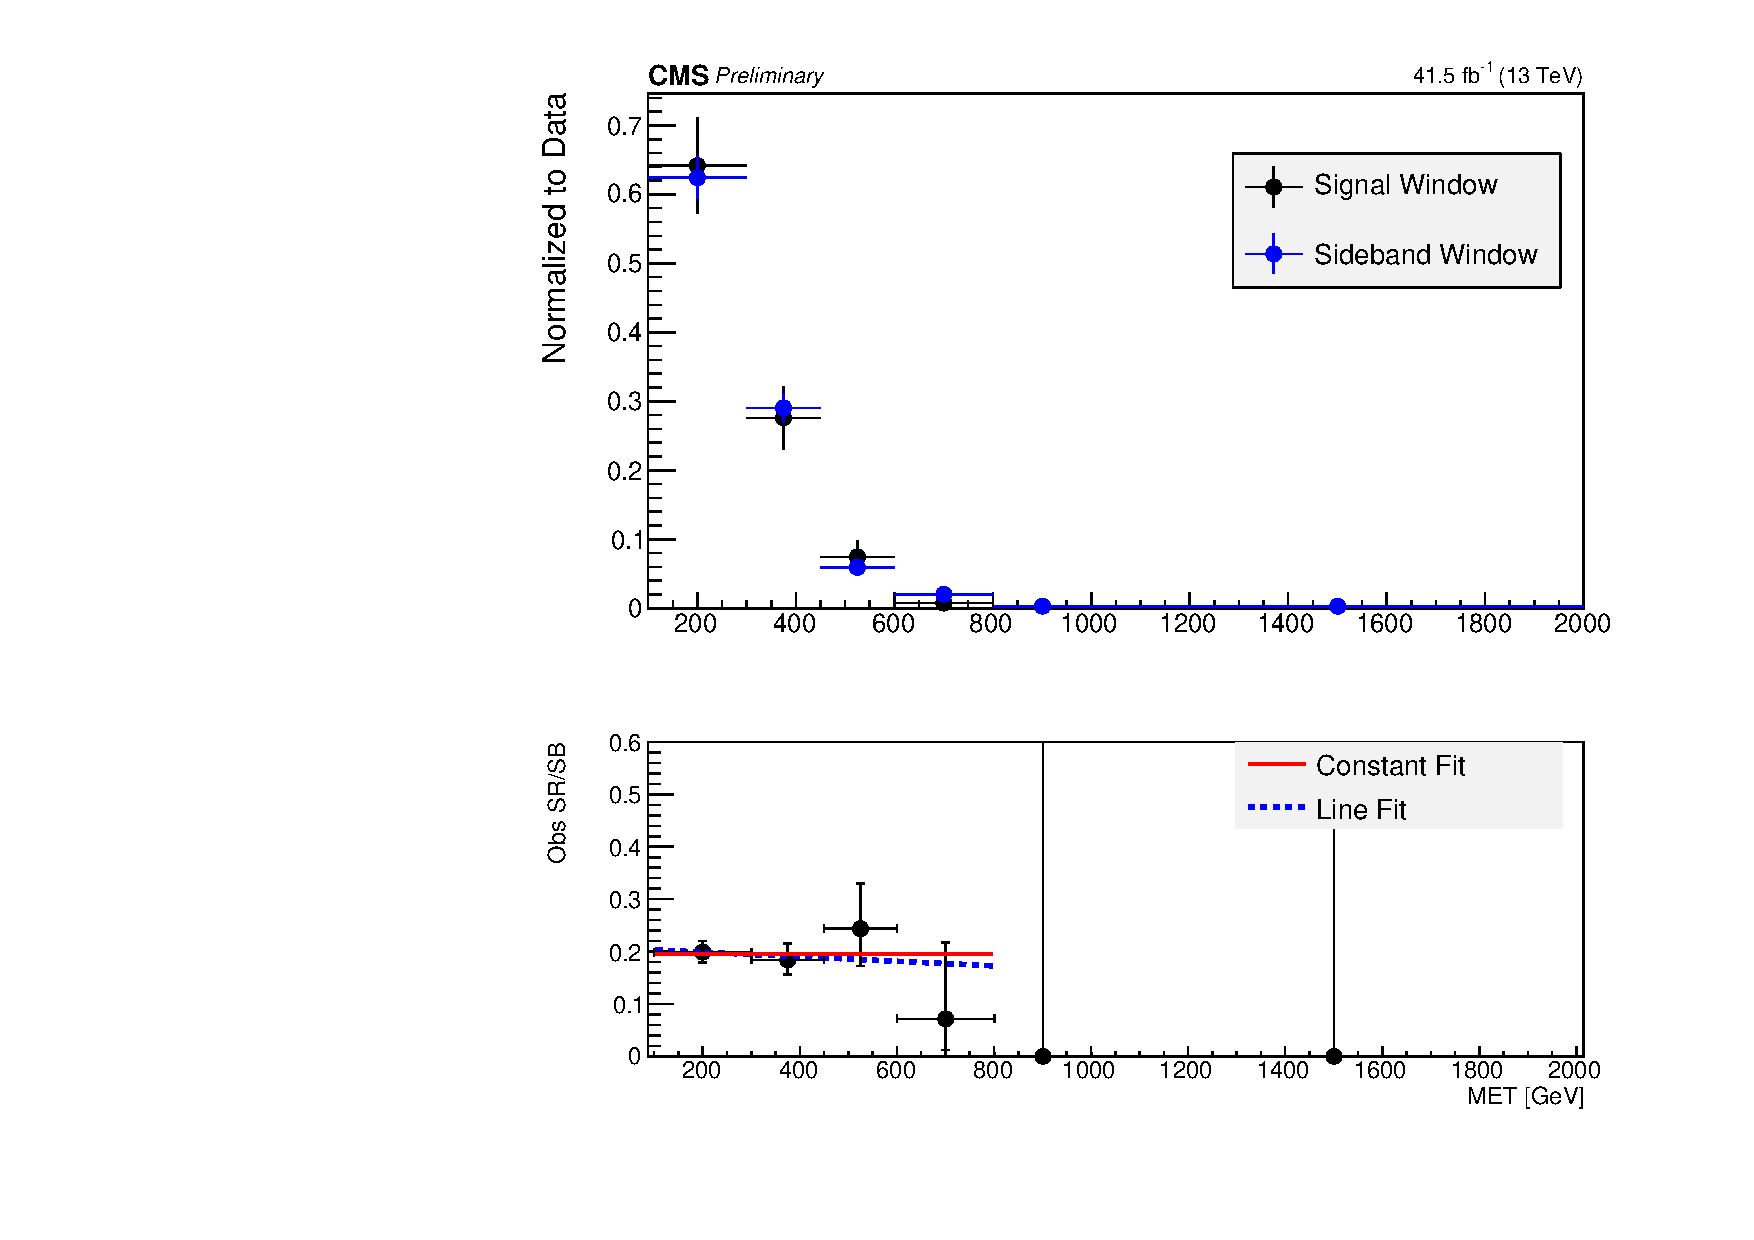
\includegraphics[trim={5px 5px 5px 5px},clip,width=0.48\linewidth]{plots/bkgestimation/Data2017SingleLepton.pdf}
    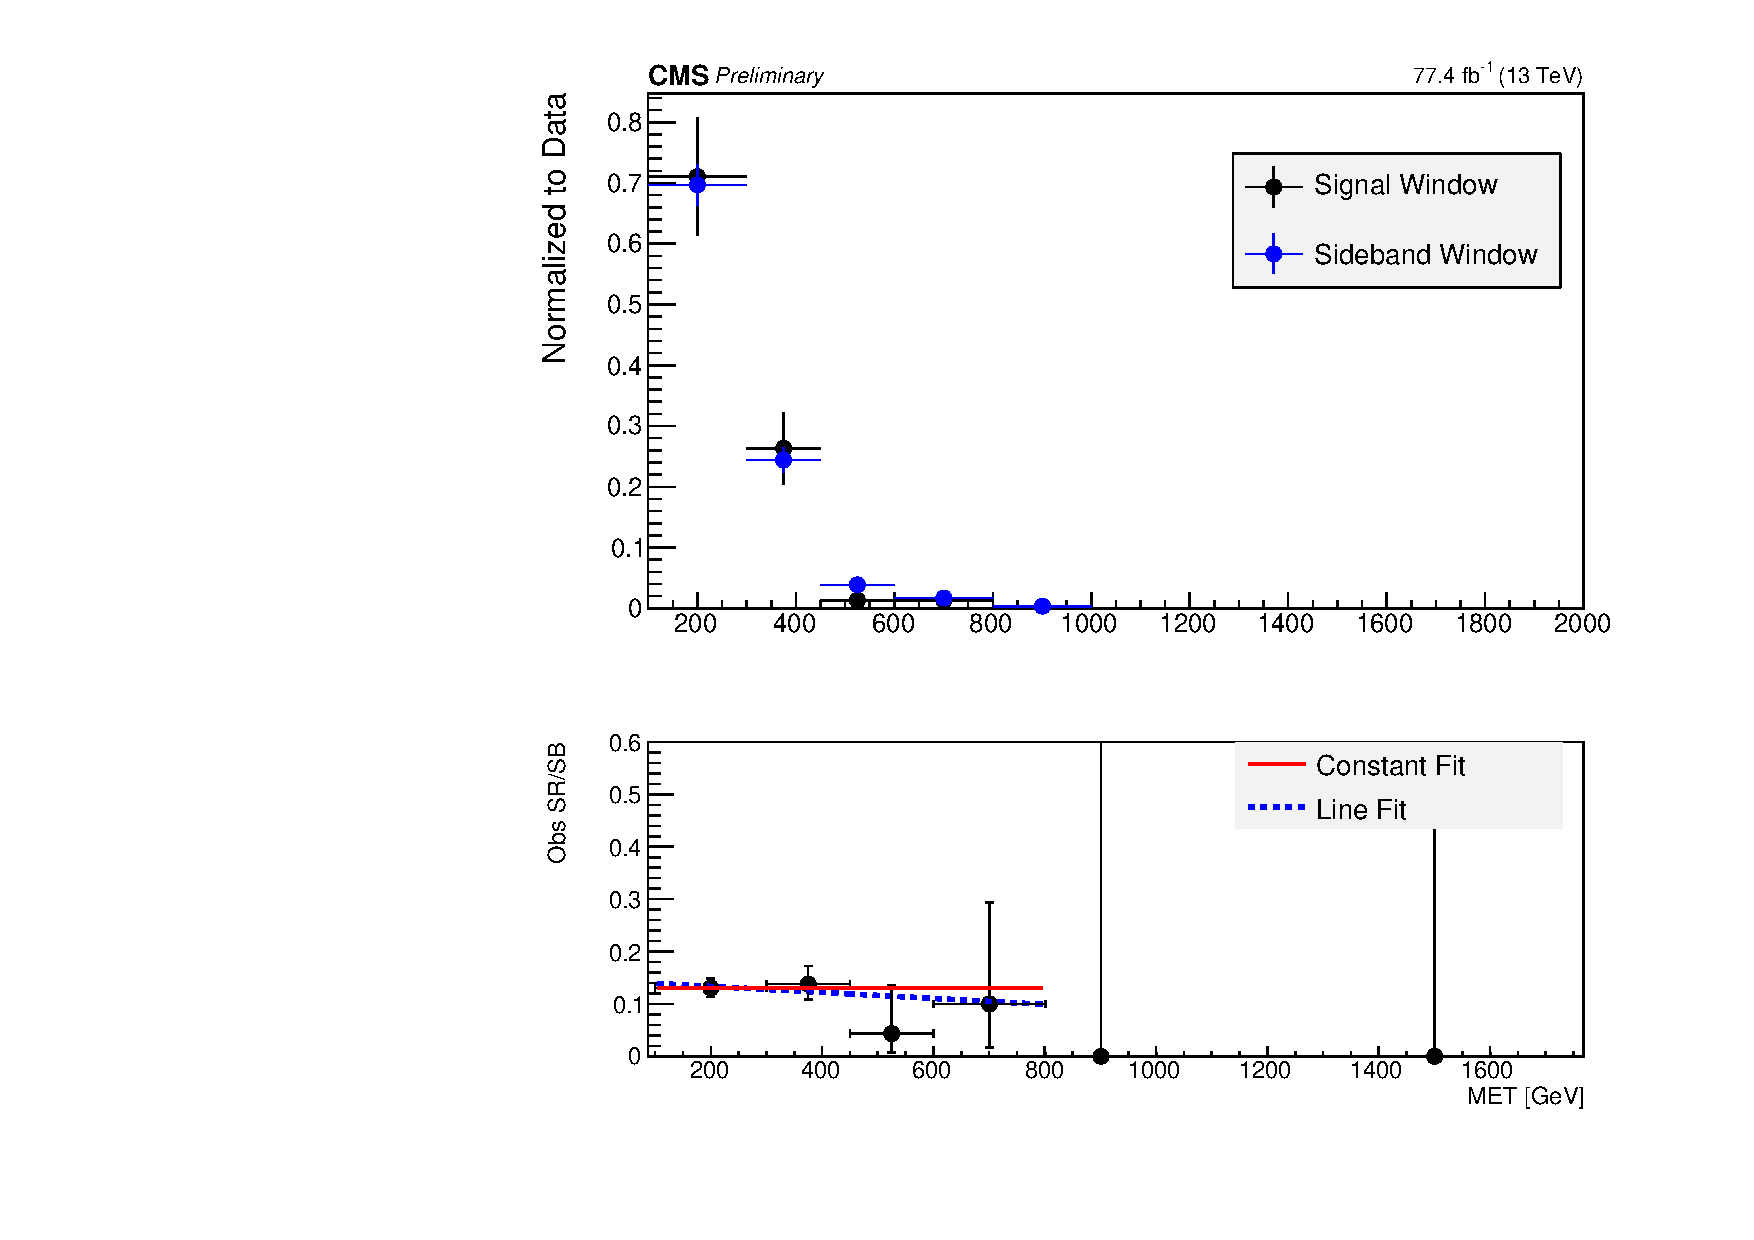
\includegraphics[trim={5px 5px 5px 5px},clip,width=0.48\linewidth]{plots/bkgestimation/Data2018SingleLepton.pdf}
    \caption{single photon validation region from 3 eras of 2016(left), 2017(middle) and 2018(right)}
    \label{fig:DataSingleLepton}
  \end{center}
\end{figure} 

\begin{figure}[htbp!]
  \begin{center}
    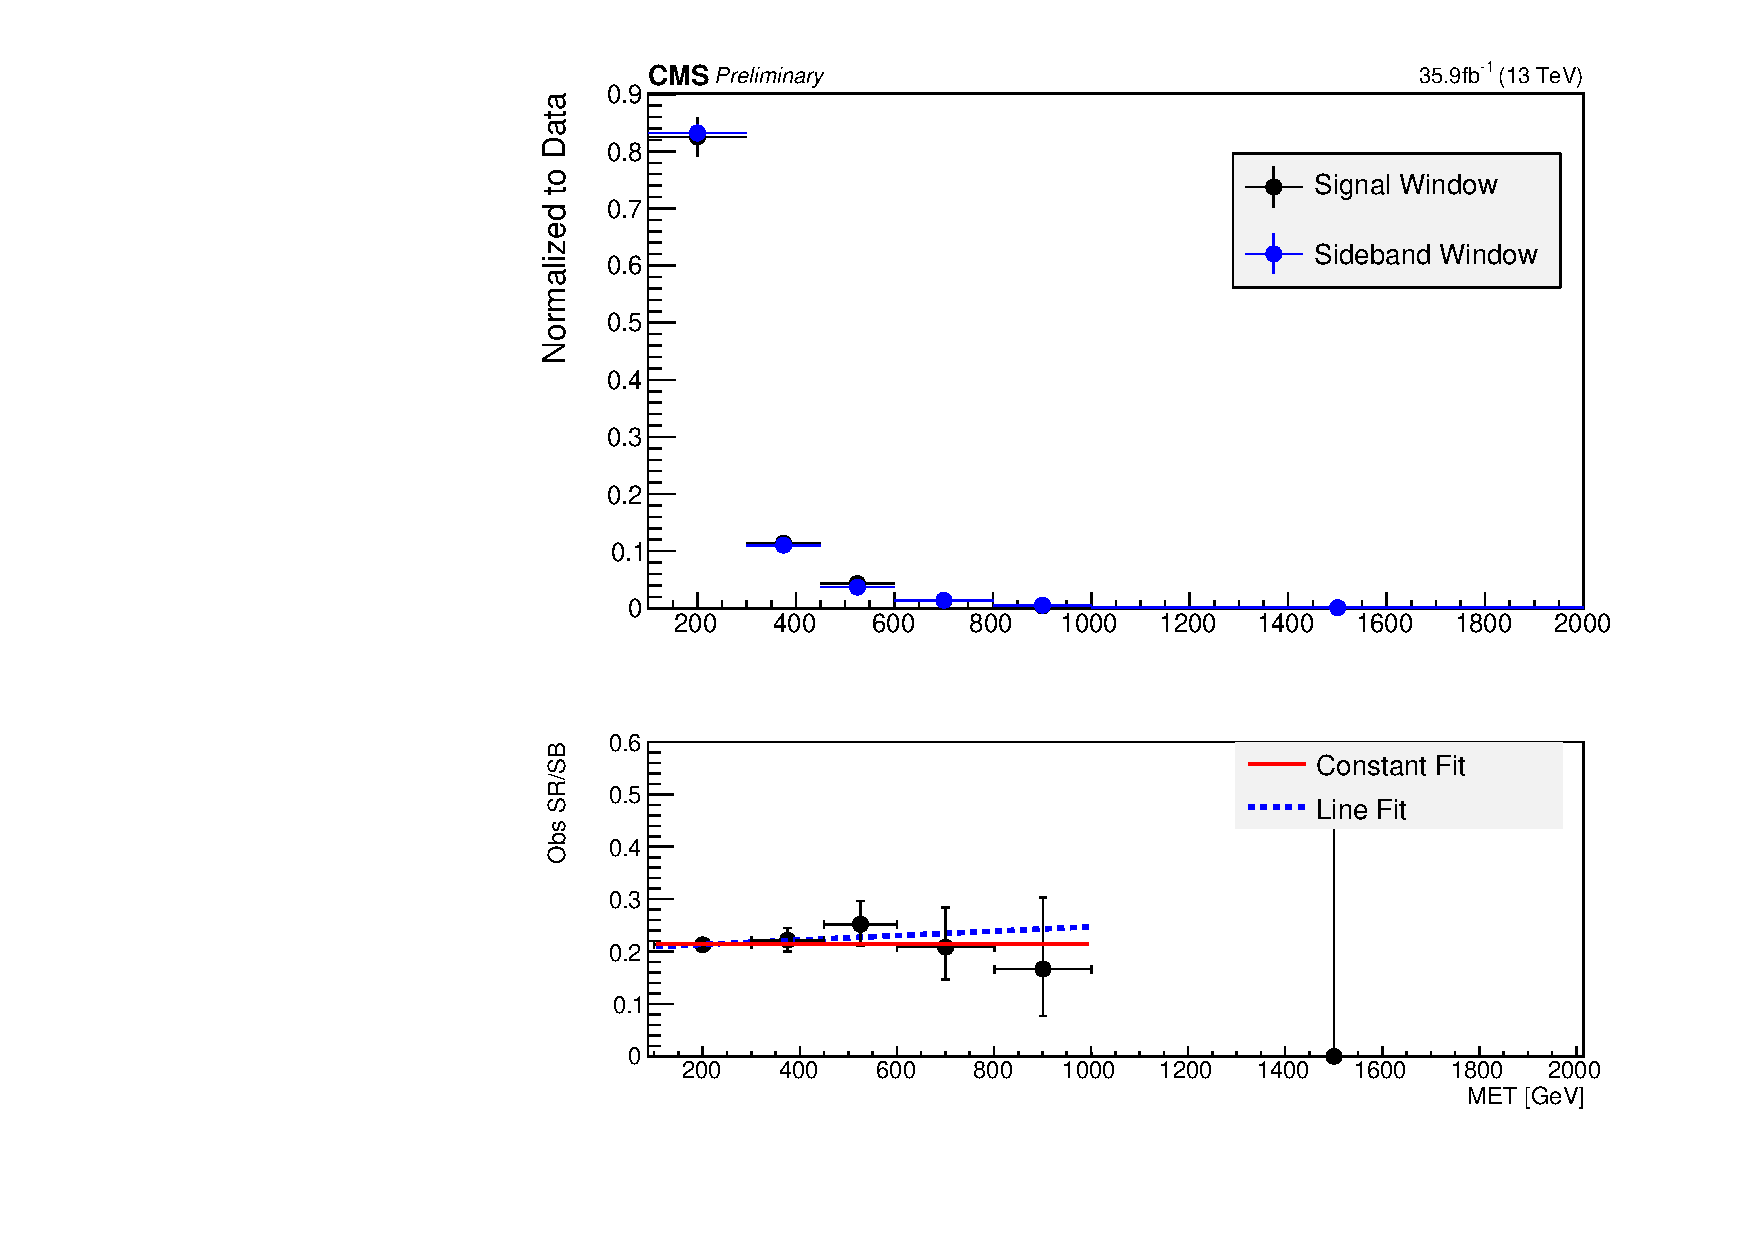
\includegraphics[trim={5px 5px 5px 5px},clip,width=0.48\linewidth]{plots/bkgestimation/Data2016SinglePhoton.pdf}\\
    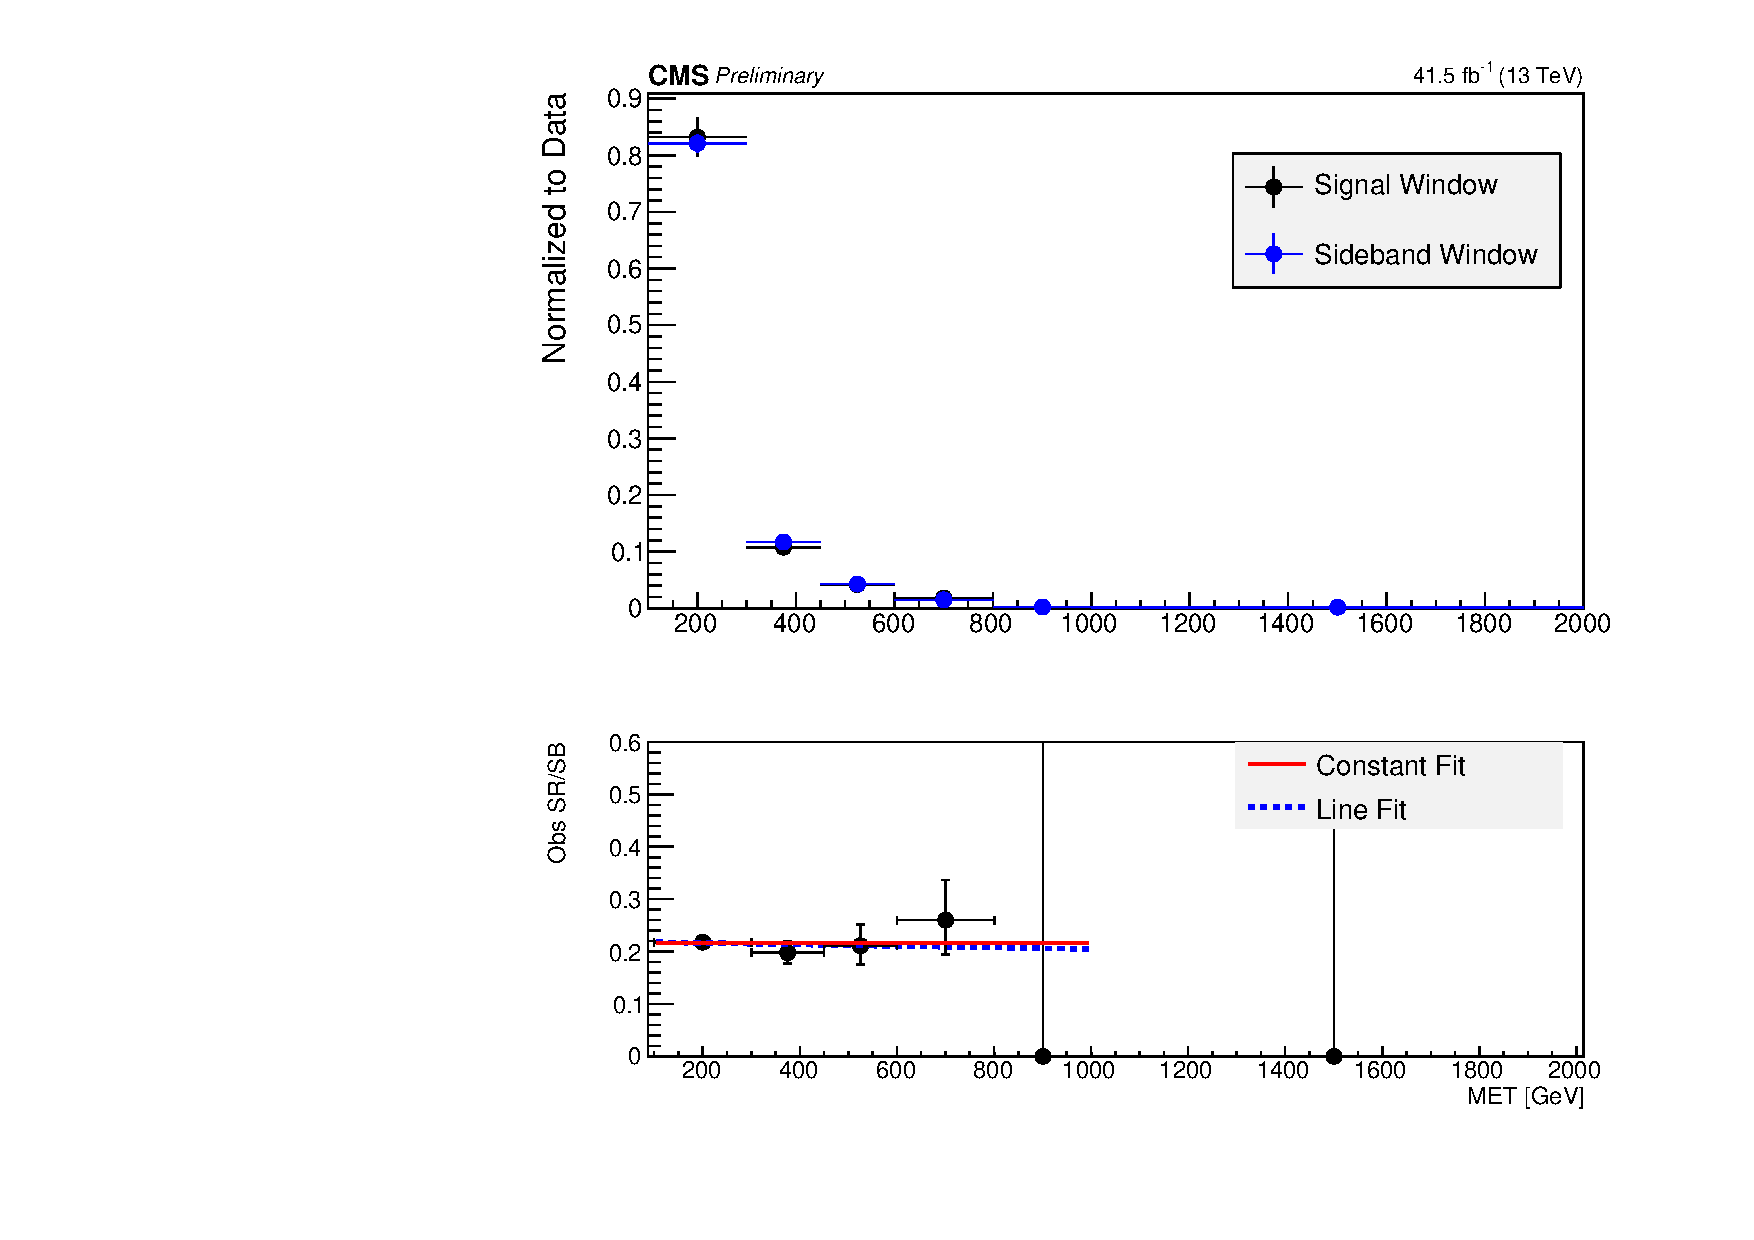
\includegraphics[trim={5px 5px 5px 5px},clip,width=0.48\linewidth]{plots/bkgestimation/Data2017SinglePhoton.pdf}
    %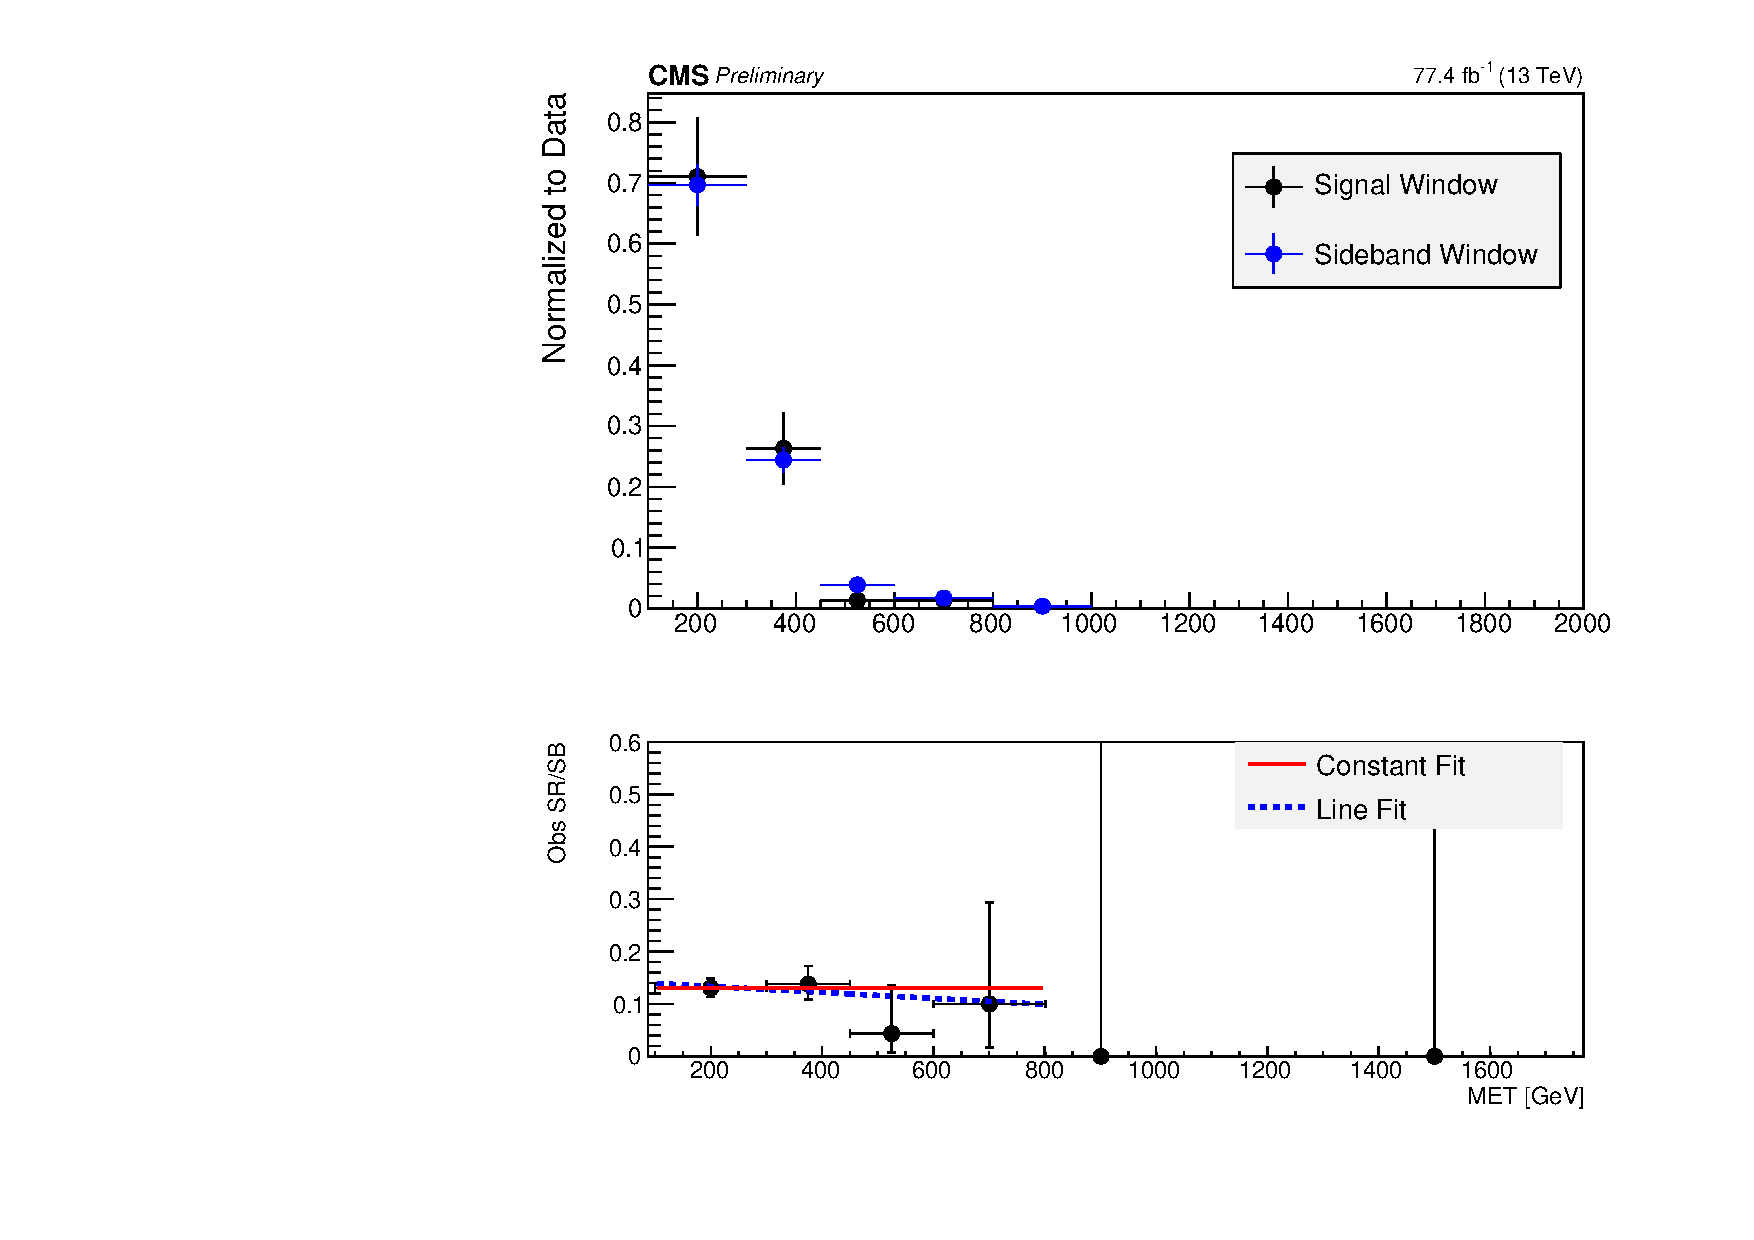
\includegraphics[trim={5px 5px 5px 5px},clip,width=0.48\linewidth]{plots/bkgestimation/Data2018SingleLepton.pdf}
    \caption{single photon validation region from 2 eras of 2016 (left) and 2017 (right)}
    \label{fig:DataSinglePhoton}
  \end{center}
\end{figure} 

\begin{figure}[htbp!]
  \begin{center}
    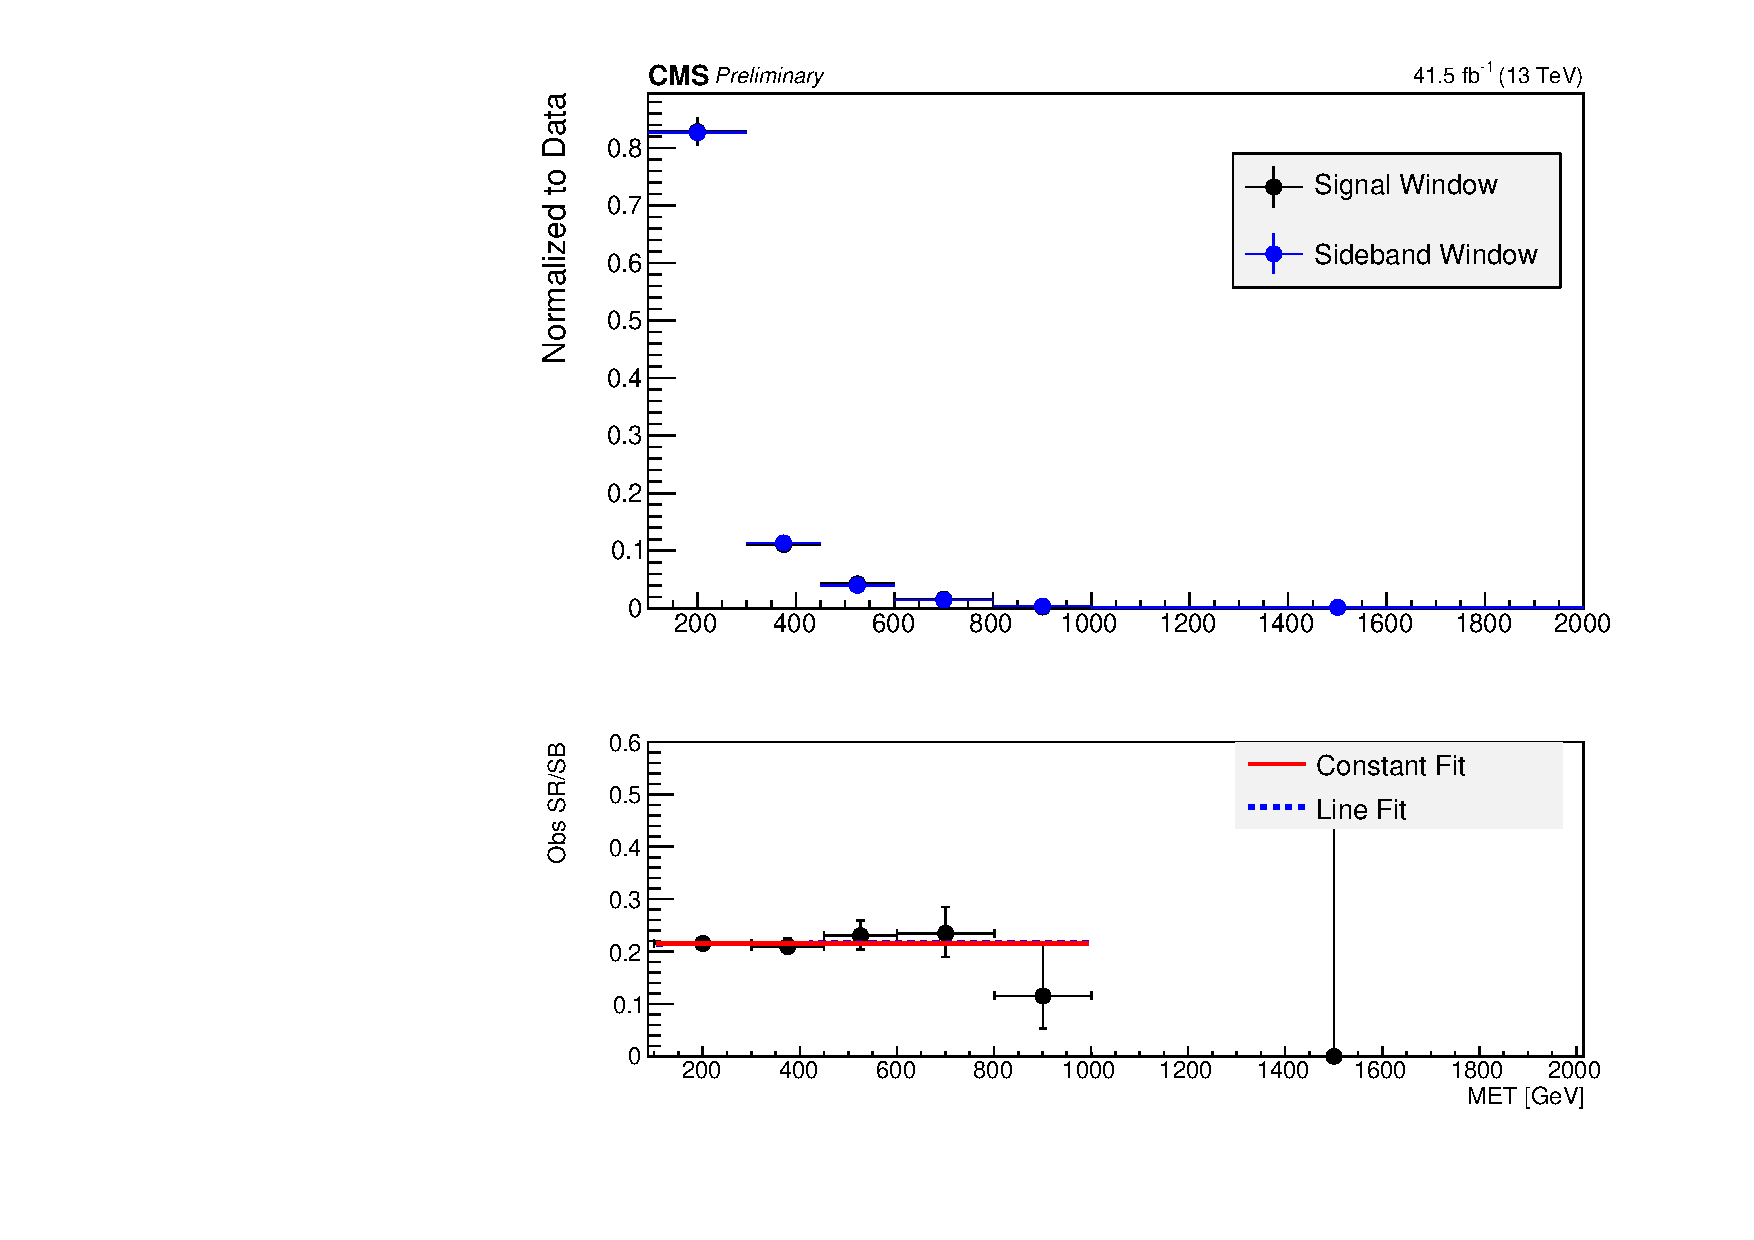
\includegraphics[trim={5px 5px 5px 5px},clip,width=0.48\linewidth]{plots/bkgestimation/DatacombinedSinglePhoton.pdf}\\
    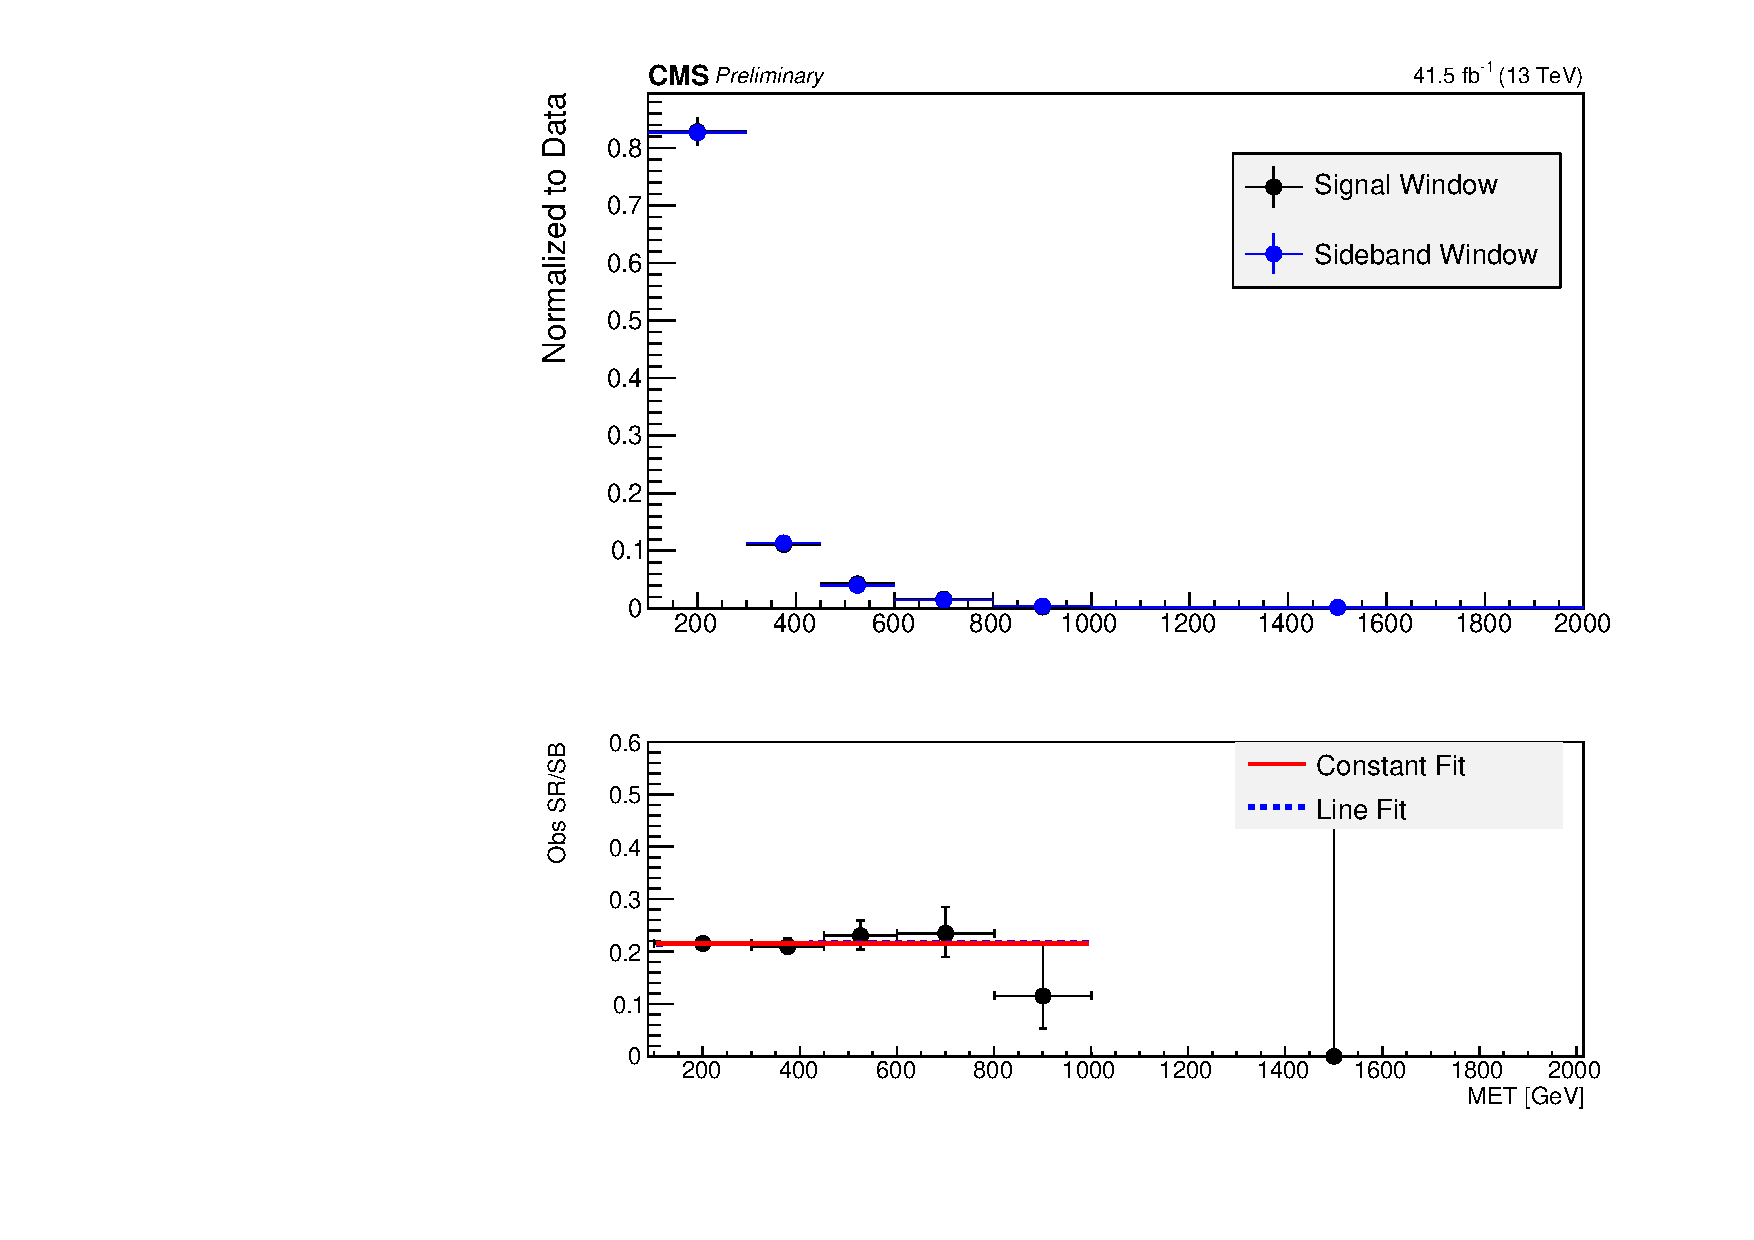
\includegraphics[trim={5px 5px 5px 5px},clip,width=0.48\linewidth]{plots/bkgestimation/DatacombinedSinglePhoton.pdf}
    \caption{combined limit for all eras of dataset for single lepton (left) and single photon (right)}
    \label{fig:DataCombinedSingleLepton}
  \end{center}
\end{figure}

\subsection{Background Systematics}
\label{sec:bkgSystematics}
 

\section{Results}
\label{sec:results}



\begin{table}[htbp!]
\caption{Predictions in the signal regions}
\centering
\begin{tabular}{c|c|c|c|c|c|}
\hline \hline
\MET bin & Uncertainty from MET shape & Uncertainty from mass shape & Total Pred. & Obs. & T5ZZ(1700) \\
\hline \hline
 $\MET[300,450]$ & $18.05 \pm 3.39$  & $0.98 \pm 0.11$ & $17.68 \pm 3.85$ & 15 & 0.24 & 0.75  \\ \hline 
 $\MET[450,600]$& $4 \pm 1.54$ & $0.86 \pm 0.16$ & $3.44\pm 1.47$ &  2  & 0.32 & 0.98 \\\hline
 $\MET[600,800]$&  $0.71 \pm 0.50$  &  $0.86 \pm 0.17$ & $0.61\pm 0.45$ &  1 & 2.13 & 4.34\\\hline
 $\MET[800,1000]$ & $18.05 \pm 3.39$  & $0.98 \pm 0.11$ & $17.68 \pm 3.85$ & 15 & 0.24 & 0.75  \\ \hline 
 $\MET>1000$& $4 \pm 1.54$ & $0.86 \pm 0.16$ & $3.44\pm 1.47$ &  2  & 0.32 & 0.98 \\\hline
\hline
\end{tabular}
\label{tab:DataPred}
\end{table}


\begin{figure}[htbp!]
  \begin{center}
    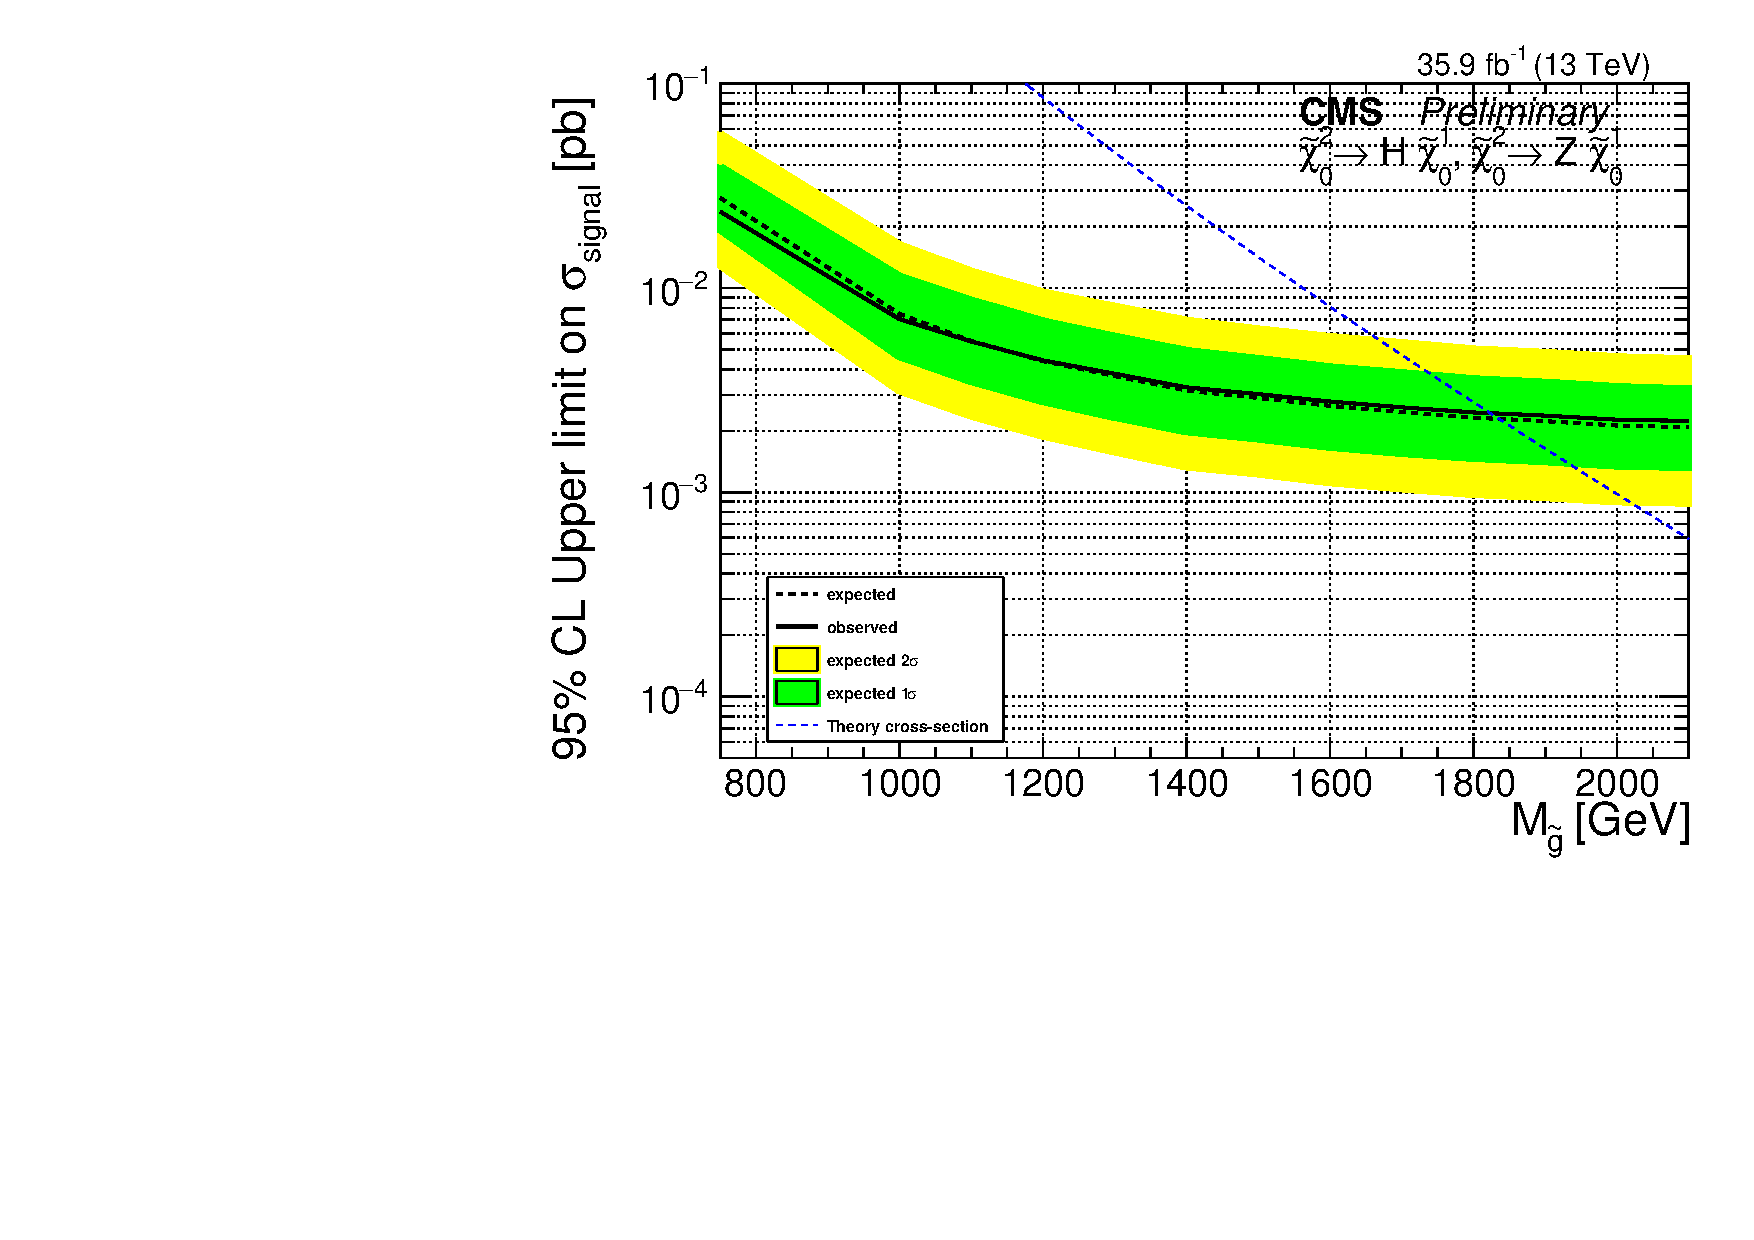
\includegraphics[width=0.6\linewidth]{plots/results/brazilT5HZResults.pdf}
    \caption{$95\%$ CL limit for the signal model considered in this analysis:  100$\%$ branching fraction to the Z boson
    }
    \label{fig:LimitsT5HH}
  \end{center}
\end{figure}


\clearpage
%\newpage
\bibliography{auto_generated}   % will be created by the tdr script.
\clearpage
\appendix
\clearpage
%%% DO NOT ADD \end{document}!

